\documentclass[10pt,twocolumn]{article}

\usepackage{CJKutf8}
\usepackage{indentfirst}
\usepackage{amsmath}

\usepackage{multirow}
\usepackage{tabularx}
% \usepackage{hyperref}
\usepackage{url}

\newcolumntype{V}{>{\raggedright\arraybackslash}X}
\newcolumntype{Y}{>{\centering\arraybackslash}X}
\newcolumntype{Z}{>{\raggedleft\arraybackslash}X}

\newcolumntype{v}{>{\hsize=.5\hsize}V}
\newcolumntype{y}{>{\hsize=.5\hsize}Y}
\newcolumntype{z}{>{\hsize=.5\hsize}Z}

\usepackage[
  top=25mm,
  bottom=19mm,
  left=19mm,
  right=19mm,
  textwidth=175mm,
  textheight=226mm,
  columnsep=8mm
]{geometry}
\usepackage{amsmath}
\usepackage{caption}
\usepackage{etoolbox}
\usepackage{titlesec}
\usepackage{ragged2e}
\usepackage{CJKutf8}
% Figures
\usepackage{subcaption}
\usepackage{float}
\usepackage[justification=raggedright]{caption}	% makes captions ragged right - thanks to Bryce Lobdell
\usepackage{lscape}                                         % Useful for wide tables or figures.
\usepackage{ragged2e}

% Algorithm
\usepackage[lined,ruled,linesnumbered]{algorithm2e}

% Table and list
\usepackage{booktabs}                   % Publication quality tables
\usepackage{multirow}

\usepackage{paralist}
\usepackage{enumitem}

% Math
\usepackage{bm}                          % Make bold, italic math symbols
\usepackage{epsfig}                      % for figures
\usepackage{graphicx}                  % another package that works for figures
\usepackage{times}
\usepackage{mathptmx}
\usepackage{mathtools}
\usepackage{amssymb,amsmath}   % Short math guide for LaTeX ftp://ftp.ams.org/pub/tex/doc/amsmath/short-math-guide.pdf

% Fonts
\usepackage{units}
\usepackage{color}

% Comments
\usepackage{comment}

% Hyperlinks
\usepackage{url}  % Hyphenation of URLs.
\usepackage[pagebackref=true,breaklinks=true,letterpaper=true,colorlinks,bookmarks=false]{hyperref}

% \usepackage{slashbox}
\usepackage{cite}
\usepackage{xspace}
\usepackage[table]{xcolor}
\usepackage{setspace}
\usepackage[percent]{overpic}
\usepackage{nccbbb}
% \usepackage{times,color}
% \usepackage{parskip}
% %\usepackage{epsfig}
% %\usepackage{psfig}
% %\usepackage[pdftex]{graphicx} % new acmsiggraph.cls
\usepackage{ifthen}
% %\usepackage[draft]{hyperref} % new acmsiggraph.cls


\renewcommand{\refname}{}  % 禁用自動 "References"
\renewcommand{\figurename}{Fig.}  % 將 "Figure" 改為 "Fig."
% 緊縮條目間距
\patchcmd{\thebibliography}{\settowidth}
  {\setlength{\itemsep}{0pt plus 0.3ex}%
   \setlength{\parskip}{0pt}%
   \settowidth}{}{}
% Macros - Jia-Bin Huang (jbhuang@vt.edu)

\renewcommand{\baselinestretch}{1}       % for squeezing the draft into the page limit, do not use

% =========================================
% Useful macros
% =========================================

% Latin abbreviations
\def\etal{et al.~}			  % and others, and co-workers
% \newcommand\etal{et al.~}
\def\eg{e.g.,~}               % for example
\def\ie{i.e.,~}               % that is, in other words
\def\etc{etc}                 % and other things, and so forth
\def\cf{cf.~}                 % compare
\def\viz{viz.~}               % namely, precisely
\def\vs{vs.~}                 % against


% Math related
\DeclareMathOperator*{\argmin}{\arg\!\min} 
\DeclareMathOperator*{\argmax}{\arg\!\max}

% Consistent margin adjustment for paragraphs, figures, and sections
\newlength\paramargin
\newlength\figmargin
\newlength\secmargin
\newlength\figcapmargin

\setlength{\secmargin}{0.0mm}
\setlength{\paramargin}{0.0mm}
\setlength{\figmargin}{0.0mm}
\setlength{\figcapmargin}{0.5mm}

\setlength{\parskip}{0pt}     % 段落間距 0
\setlength{\parindent}{1em}   % 段落開頭縮排（1em 可調）

\newcommand{\red}{\textcolor{red}}
\newcommand{\blue}{\textcolor{blue}}

% minipage
\newcommand{\mpage}[2]
{
\begin{minipage}{#1\linewidth}\centering
#2
\end{minipage}
}

\newcommand{\mfigure}[2]
{
\begin{subfigure}[b]{#1\linewidth}\centering
\includegraphics[width=\linewidth]{#2}
\end{subfigure}
}


\newcommand{\Paragraph}[1]
{
\vspace{\paramargin}
\paragraph{#1}
}

\newcommand{\heading}[1]
{
\vspace{1mm}
\noindent \textbf{#1}
}   

% References for figures, tables, equations, and sections
\newcommand{\secref}[1]{Section~\ref{sec:#1}}
\newcommand{\figref}[1]{Figure~\ref{fig:#1}} 
\newcommand{\tabref}[1]{Table~\ref{tab:#1}}
\newcommand{\eqnref}[1]{Equation~\ref{eq:#1}}
\newcommand{\thmref}[1]{Theorem~\ref{#1}}
\newcommand{\prgref}[1]{Program~\ref{#1}}
\newcommand{\algref}[1]{Algorithm~\ref{#1}}
\newcommand{\clmref}[1]{Claim~\ref{#1}}
\newcommand{\lemref}[1]{Lemma~\ref{#1}}
\newcommand{\ptyref}[1]{Property~\ref{#1}}

% Comments
\long\def\ignorethis#1{}
\newcommand {\jiabin}[1]{{\color{blue}\textbf{Jia-Bin: }#1}\normalfont}
\newcommand {\james}[1]{{\color{violet}\textbf{James: }#1}\normalfont}
\newcommand {\eric}[1]{{\color{magenta}\textbf{Eric: }#1}\normalfont}
\newcommand {\todo}{{\textbf{\color{red}[TO-DO]\_}}}
\def\newtext#1{\textcolor{blue}{#1}}
\def\modtext#1{\textcolor{red}{#1}}
\newcommand{\note}[1]{{\it\color{blue} #1}}

\newcommand{\tb}[1]{\textbf{#1}}
\newcommand{\mb}[1]{\mathbf{#1}}

\newcommand{\jbox}[2]{
  \fbox{%
  	\begin{minipage}{#1}%
  		\hfill\vspace{#2}%
  	\end{minipage}%
  }}

\newcommand{\jblock}[2]{%
	\begin{minipage}[t]{#1}\vspace{0cm}\centering%
	#2%
	\end{minipage}%
}


% \titleformat{\section}
%   {\normalfont\bfseries\centering}
%   {\thesection.}{1em}{}

% % 將 \subsection 調成 10pt 加粗
% \titleformat{\subsection}
%   {\normalsize\bfseries} % 10pt = \normalsize
%   {\thesubsection.}{1em}{}

% % 格式設定：斜體、不加粗、10pt、編號、左對齊
% \titleformat{\subsubsection}
%   {\normalsize\itshape}      % 10pt, 斜體
%   {\thesubsubsection.}       % 顯示 5.1.1. 編號
%   {1em}                      % 編號與文字之間距
%   {}                         % 不加其他

% % 間距設定：上間距1ex，下間距0.3ex（很緊湊）
% \titlespacing*{\subsubsection}
%   {0pt}       % 左邊距
%   {1.5ex plus .3ex minus .3ex}  % 上方距離
%   {0.3ex}     % 下方距離（正文與標題之間）

% --- Section 樣式設定 ---
\titleformat{\section}
  {\normalsize\bfseries\centering} % 10pt 粗體 置中
  {\thesection.}{0.25em}{}

\titlespacing*{\section}
  {0pt}{1.2em}{0.8em} % 上下空白（可調整為更精確 10pt 單位）

% --- Subsection 樣式設定 ---
\titleformat{\subsection}
  {\normalsize\bfseries}  % 10pt 粗體 左對齊
  {\thesubsection.}{0.25em}{}

\titlespacing*{\subsection}
  {0pt}{1.2em}{0.5em}

% --- Subsubsection 樣式設定 ---
\titleformat{\subsubsection}
  {\normalsize\itshape}  % 10pt 斜體 左對齊
  {\thesubsubsection.}{0.25em}{}

\titlespacing*{\subsubsection}
  {0pt}{1.2em}{0.3em}
% Define math symbols that appear in the texts


\def\grayimg{X}                 % input grayscale image
\def\predimg{Y}                 % predicted color image
\def\predGT{\predimg^{GT}}      % ground truth color image
\def\instngray{\grayimg_i}      % instance image
\def\instnpred{\predimg_i}      % colorized instance image
\def\instnGT{\predimg^{GT}_i}   % ground truth instance image
\def\instnbox{B}                % set of instance object bounding boxes
\def\instnboxi{\instnbox_i}     % single instance object bounding box
\def\fullmodel{M_F}                 % full-image colorization model
\def\instnmodel{M_I}                % instance colorization model
\def\fusemodule{F_j}                % j-th fusion module
\def\fullfetr{f^{\grayimg}_j}       % full-image feature at j-th layer
\def\instnfetr{f^{\instngray}_j}    % instance feature at  j-th layer
\def\resizedInstnfetr{\Bar{f^{\instngray}_j}}    % resized instance feature at  j-th layer
\def\fusedfetr{f^{\tilde{\grayimg}}_j}  % fused full-image feature at j-th layer
\def\fullweight{W_F}                % full-image weight map
\def\instnweight{W^{i}_I}           % instance weight map
\def\resizedInstnweight{\Bar{W^{i}_I}}           % resized instance weight map
\def\colorspace{$\mathrm{CIE}~\mathrm{L^{\ast}a^{\ast}b^{\ast}}$}

% ===== old =====
% \def\gray{X}
% \def\colordomain{Y}
% \def\xi{\gray_i}
% \def\yi{\colordomain_i}
% \def\instancebb{B}
% \def\bi{\instancebb_i}
% \def\fm{M_F}
% \def\instam{M_I}
% \def\objm{M_O}
% \def\fum{F_l}


\graphicspath{{figure}, {images}, {example}}

\captionsetup[figure]{font=small}
\captionsetup[table]{font=small}

\date{}

% Support for easy cross-referencing
\usepackage[capitalize]{cleveref}
\crefname{section}{Sec.}{Secs.}
\Crefname{section}{Section}{Sections}
\Crefname{table}{Table}{Tables}
\crefname{table}{Tab.}{Tabs.}

\begin{document}
\pagestyle{empty} % 拿掉頁碼


% \title{\textbf{ON THE IMPORTANCE OF BACKBONE, PRETRAINING AND HYPERPARAMETER SELECTION FOR HIERARCHICAL FINE-GRAINED IMAGE RECOGNITION}}
% \title{\textbf{A SYSTEMATIC STUDY ON BACKBONE, \\ PRETRAINING AND TRANSFERABILITY FOR \\ HIERARCHICAL FINE-GRAINED IMAGE RECOGNITION}}
\title{\textbf{Revisiting the Backbone, Pretraining and Transferability for \\ Hierarchical Fine-Grained Image Recognition}}
% for chinese text
% \AtBeginDocument{\begin{CJK}{UTF8}{bkai}} % 使用標楷體    
% \AtEndDocument{\clearpage\end{CJK}}
\begin{CJK}{UTF8}{bkai}
\author{
    Augusto Christian Surya (蘇立光)$^{1}$\thanks{Equal contribution.}, 
    Edwin Arkel Rios (冉恩達)$^{2}$\footnotemark[1],\\
    Bo-Cheng Lai (賴伯承)$^{2}$,
    Min-Chun Hu (胡敏君)$^{1}$\\
    \\
    $^{1}$Department of Computer Science, National Tsing Hua University, Hsinchu, Taiwan\\
    $^{2}$Department of Electronics Engineering, National Yang Ming Chiao Tung University, Hsinchu, Taiwan\\
    E-mails: ss110000162@gapp.nthu.edu.tw, edwinarkel.rios@gmail.com, \\
    bclai@nycu.edu.tw, anitahu@cs.nthu.edu.tw
}

\maketitle

\end{CJK}

\thispagestyle{empty}  % 保險再加一行拿掉頁碼1


\begin{center}
\textbf{ABSTRACT}
\end{center}

\noindent
Fine-grained image recognition (FGIR) is a task that requires models to distinguish visually similar subcategories within a broader class. FGIR tasks are naturally organized into hierarchical structures where coarse-level groupings provide valuable semantic context for fine-level classification. Despite this, most prior work in hierarchical FGIR evaluates only a limited set of backbone architectures, leaving the influence of backbone and pretraining largely underexplored. This gap is critical, as the backbone determines the quality of feature representations used across multiple classification heads in hierarchical settings. In this work, we systematically study 21 pretrained models, including convolutional and transformer-based backbones, under full fine-tune and frozen backbone settings. We also evaluate 18 transferability metrics to examine their ability to predict performance. Our results show that backbone and hyperparameter selection heavily influence FGIR performance; ResNets pretrained with discriminative objectives, such as MoCov3 and SwaV, display high mean accuracy and low standard deviation, making them suitable as backbones for development of future hierarchical fine-grained applications. Most of the metrics display weak or inconsistent correlation with transfer accuracy across different settings, highlighting an open challenge for future research.

\noindent
\begin{flushleft}
\justifying{\textbf{\textit{Keywords:}} Fine-Grained Object Categorization, Hierarchical Classification, IPPR, CVGIP 2025.}
\end{flushleft}

\section{INTRODUCTION}
Fine-grained image recognition (FGIR) is a computer vision task to distinguish between visually similar subcategories within a broader class. While fine-grained categories are organized into taxonomic hierarchies, early works on FGIR approaches often treat categories as flat labels\cite{zhang_part-based_2014, zheng_learning_2017}, ignoring semantic relationships between them. This limited perspective prevents models from fully leveraging hierarchical relationships, leading to suboptimal performance.\cite{chen_fine-grained_2018}

\begin{figure}[ht]
    \centering
    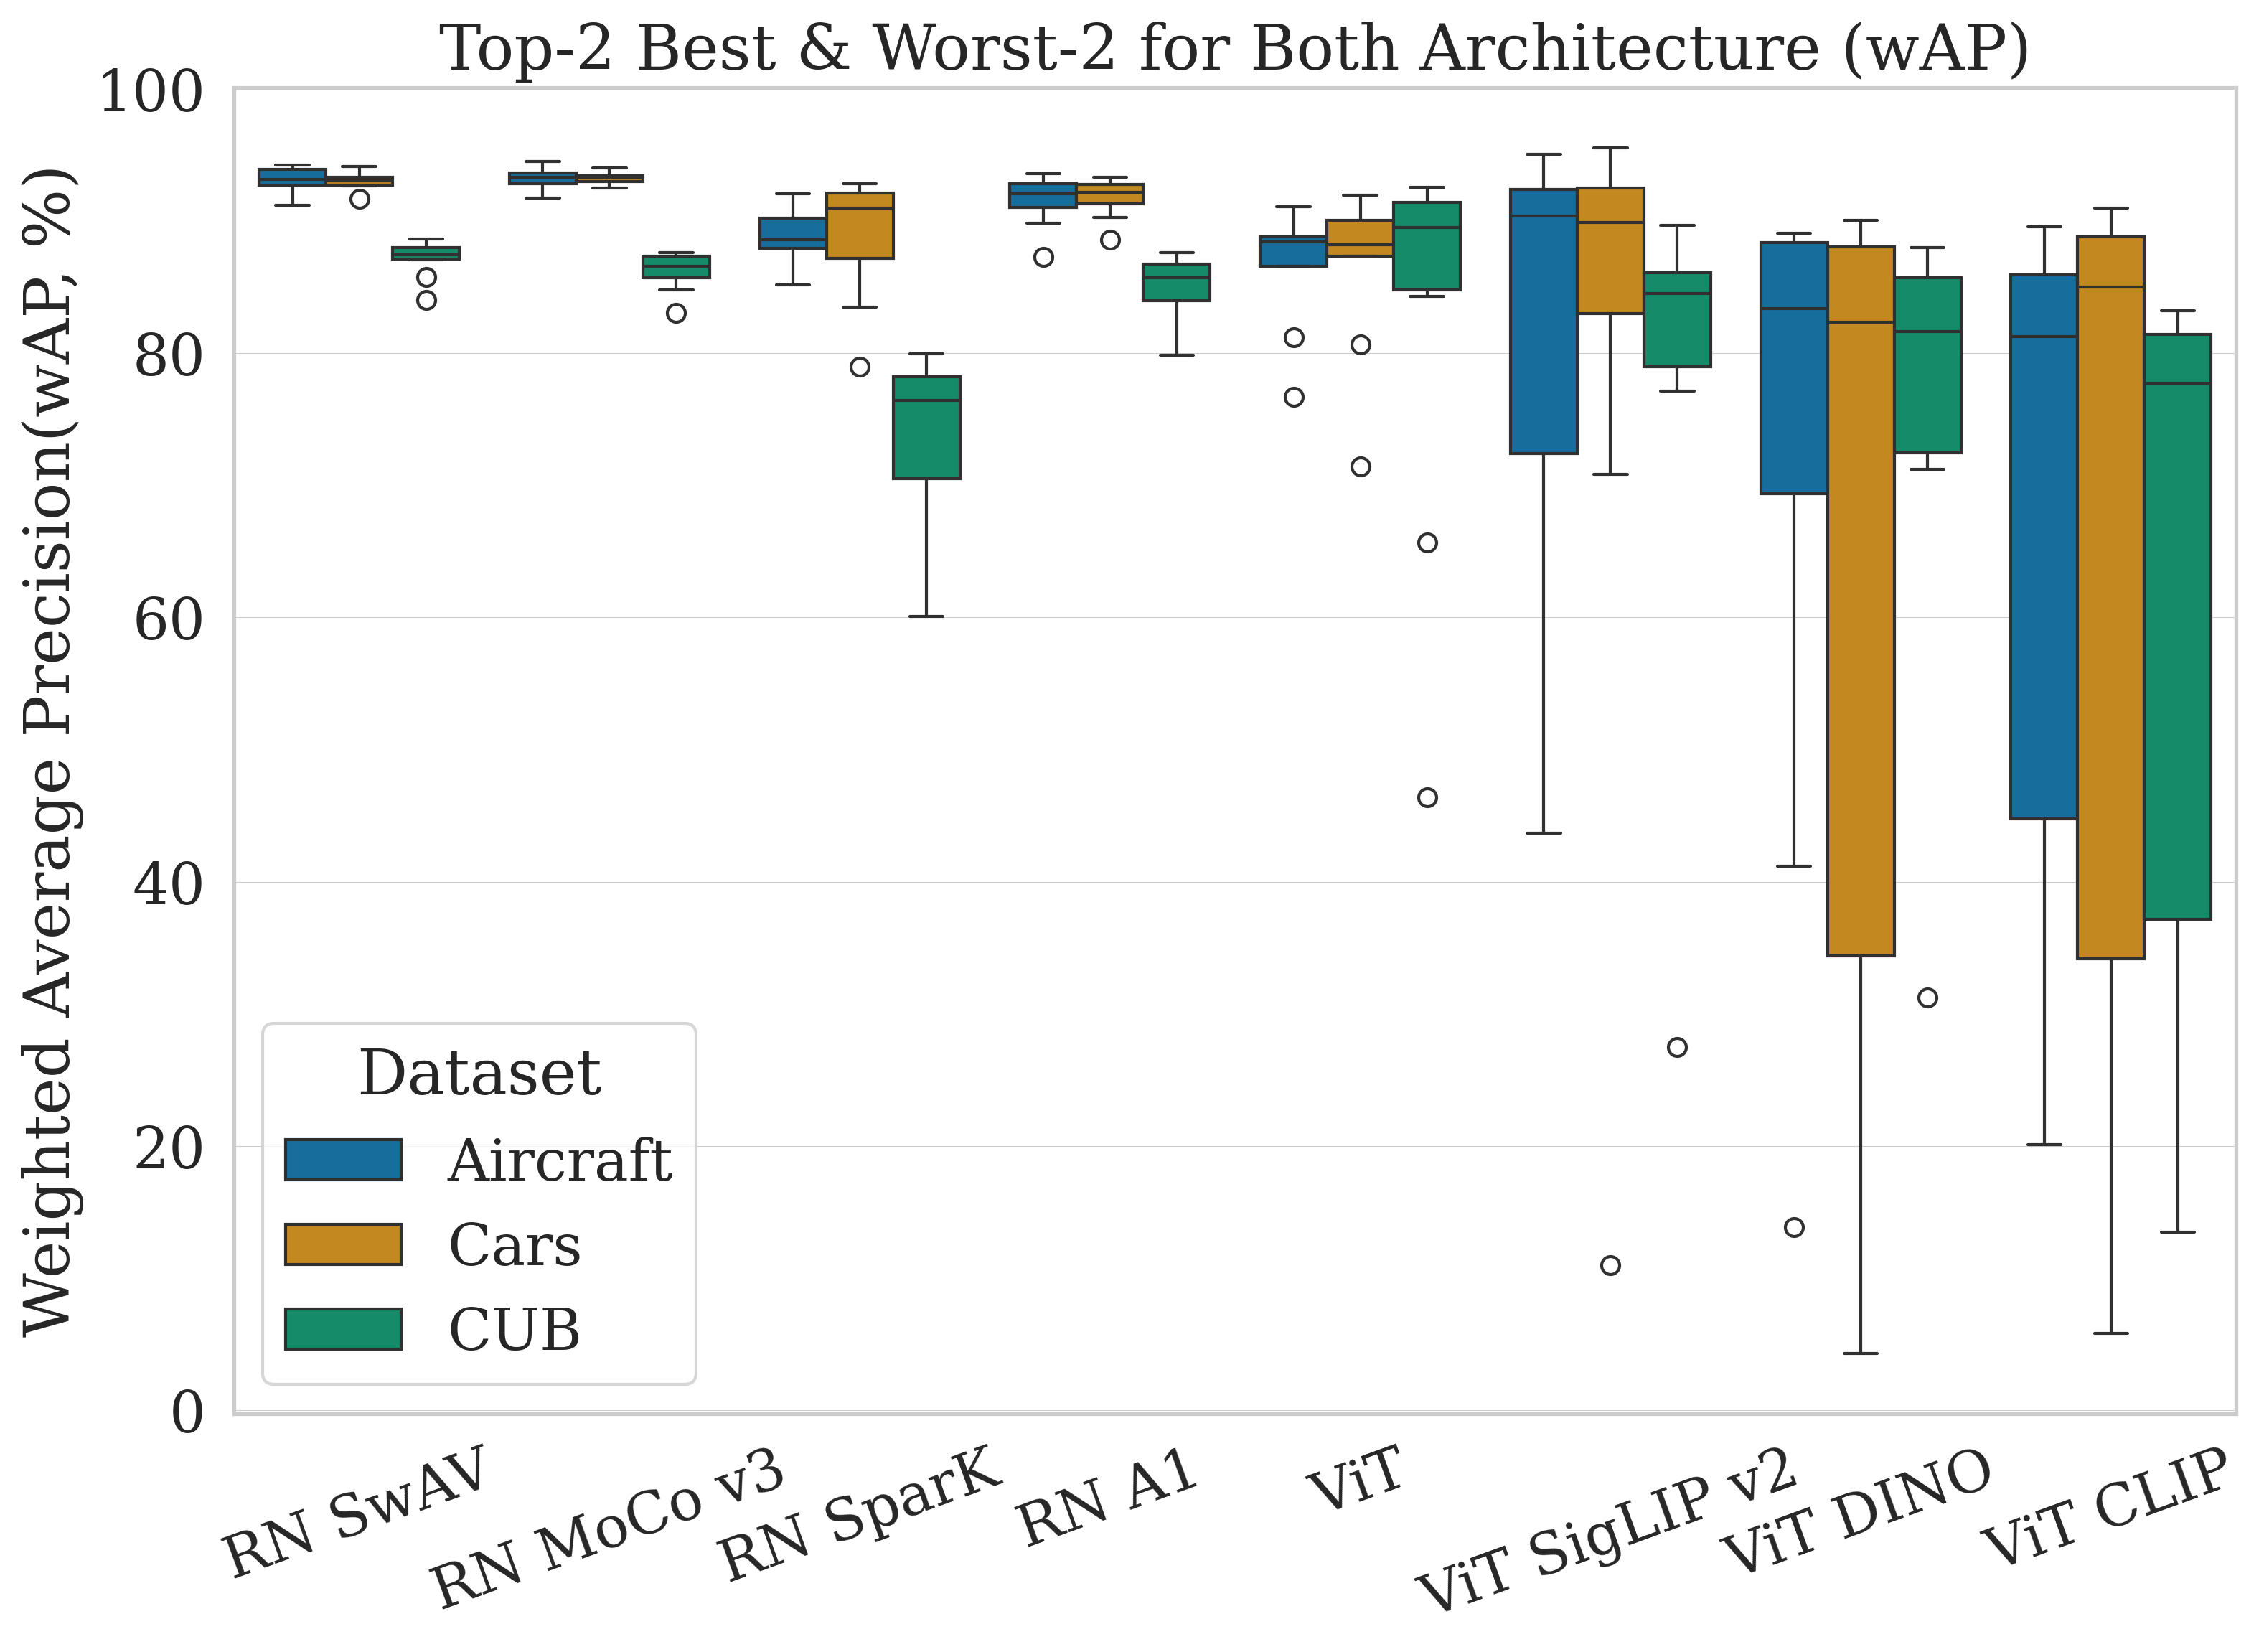
\includegraphics[width=0.95\linewidth]{figures/imgs/best_a_worst.png}
    \caption{Comparison of backbone performance. We visualize the Top-2 and Bottom-2 performing ResNet and ViT models respectively, ranked by Weighted Average Precision.}
    \label{fig:best_a_worst}
    \vspace{-0.3cm}
\end{figure}

Hierarchical FGIR addresses this limitation by leveraging semantic relationships across different levels of granularity, using information from coarse categories to enhance fine-grained classification performance. Several approaches have explored this direction, such as granularity specific classifiers \cite{chang_your_2021} and hierarchically discriminative loss functions \cite{chen_fine-grained_2018}. While these directions have shown promise, they overlook a more foundational component: the backbone itself.

Although prior work in standard FGIR has shown that different backbones can lead to a significant impact on recognition performance \cite{ye_image_2024}, the role of backbone choice in hierarchical FGIR remains underexplored. Most hierarchical FGIR methods continue to rely on a narrow set of backbones\cite{wang_multiple_2015, cerri_reduction_2016, chen_fine-grained_2018, chang_your_2021, chen_label_2022, chen_hierarchically_2024}, making it unclear whether backbone differences affect the performance in taxonomic hierarchies. This raises an important question: \textbf{To what extent does the backbone influence performance in hierarchical FGIR?}

In this work, we conduct \textbf{the first study on backbone selection for hierarchical FGIR}. We benchmark a wide range of convolutional and transformer-based models across multiple datasets and hyperparameters, showing that backbone choice alone can yield drastically different outcomes, from state-of-the-art performance(91\% wAP on CUB for base ViT), to poor results (80\% wAP on CUB for CLIP), as observed in  fig.~\ref{fig:best_a_worst}. To understand this gap, we evaluate 7 metrics from prior work~\cite{kornblith_better_2019, nayman_diverse_2022} and introduce 11 additional metrics. While effective in standard classification, many of these metrics fail to generalize to hierarchical FGIR. This \textbf{underscores a disconnect between general transferability and hierarchical recognition}, and highlights the need for better predictors, especially given the cost of exhaustive model and hyperparameter search~\cite{strubell_energy_2019, lacoste_quantifying_2019}.

Our study offers three main contributions: 
\begin{enumerate}[topsep=3pt, itemsep=2pt, parsep=1pt]
    \item We conduct an extensive study on the role of 11 CNN-based and 10 ViT-based backbone and pretraining in determining hierarchical FGIR performance. The backbone can \textbf{impact wAP by up to 11\%}.
    \item We study the impact of hyperparameters in hierarchical FGIR. Hyperparameters can make a significant \textbf{change in wAP of up to 80\%}.
    \item Our analysis of 18 predictive highlights the challenge of predicting the performance hierarchical FGIR.
\end{enumerate}

\section{RELATED WORKS}
\subsection{Fine-Grained Image Recognition(FGIR)}
Early FGIR methods relied on additional human supervision, such as bounding boxes or part annotations, to improve discriminative localization~\cite{zhang_part-based_2014}. While effective, these methods are difficult to scale due to the cost of annotations. Later approaches shifted toward using image-level labels combined with attention mechanisms to discover informative regions. For example, MA-CNN~\cite{zheng_learning_2017} automatically identified key parts without requiring part-level labels. However, these models largely ignored class hierarchies, limiting their ability to capture semantic structure and generalize across categories.

\vspace{-0.2cm}
\subsection{Hierarchical Fine-Grained Image Recognition}
To address these limitations, recent methods have incorporated multi-granularity structures into FGIR commonly referred to as *Hierarchical FGIR*. One of the first works, Multi-Granularity Descriptor (MGD)~\cite{wang_multiple_2015}, used weakly supervised taxonomic descriptors. This was followed by methods like Hierarchical Semantic Embedding (HSE)~\cite{chen_fine-grained_2018} and granularity-specific classifiers~\cite{chang_your_2021}, which introduced hierarchy-aware loss functions and multi-level prediction heads. While these approaches improved performance by leveraging taxonomic structure, they often still struggle to disambiguate classes within the same coarse category and current hierarchical FGIR methods predominantly rely on a limited subset of backbone architectures.

\vspace{-0.2cm}
\subsection{Backbone effect on FGIR}
Recent work has explored the impact of backbone architectures on transfer learning and FGIR. Kornblith et al. \cite{kornblith_better_2019} investigated whether ImageNet accuracy correlates with downstream performance on fine-grained tasks, concluding that it generalizes well. Nayman et al. \cite{nayman_diverse_2022} extended Kornblith et al.'s work by introducing alternative metrics to better predict transferability across tasks. However, both studies focus on general vision benchmarks and do not analyze hierarchical recognition explicitly, leaving open questions about how backbone design affects hierarchical FGIR.

\section{EXPERIMENT SETUP}
\subsection{Architecture Overview}
\begin{figure}[ht]
    \centering
    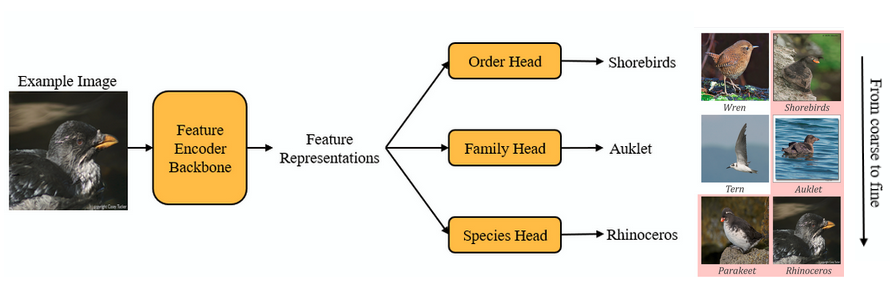
\includegraphics[width=1\linewidth]{figures/imgs/architecture.png}
    \caption{Overall Architecture of the pipeline for this experiment}
    \label{fig:architecture}
    \vspace{-0.18cm}
\end{figure}

Our architecture is based on the hierarchical pipeline of Chang et al.~\cite{chang_your_2021}. An input image is passed through a feature encoder (backbone), whose output is shared across classification heads at multiple levels of semantic granularity (Fig.~\ref{fig:architecture}). We use 2 or 3-level taxonomy, where each level has its own classifier head to predict coarse-to-fine labels.

The backbone is central to the architecture: its representational quality directly impacts the accuracy of all hierarchical predictions. By varying the backbone while keeping the rest of the pipeline fixed, we isolate and evaluate its contribution to hierarchical FGIR performance.

\subsection{Models}
We evaluate 21 pretrained models across two backbone types, \textbf{Transformer (ViT-B)} and \textbf{ResNet50}, covering a broad range of training methods, including fully supervised (FSL), semi-supervised (SemiSL), and self-supervised learning (SSL).  
Here are the exact models used:
\begin{itemize} [topsep=3pt, itemsep=2pt, parsep=1pt]
    \item \textbf{ViT-B models}:
    \begin{itemize}[topsep=3pt, itemsep=2pt, parsep=1pt]
        \item \textbf{FSL}: ViT\cite{dosovitskiy_image_2021}, DeiT\cite{touvron_training_2021}, DeiT3 (IN1K, IN21K)\cite{avidan_deit_2022}, MIIL \cite{ridnik_imagenet-21k_2021}
        \item \textbf{SSL (Discriminative)}: MoCoV3\cite{chen_empirical_2021}, DINO\cite{caron_emerging_2021}, CLIP-LAION5B\cite{cherti_reproducible_2023}, SigLIP-v2\cite{tschannen_siglip_2025}
        \item \textbf{SSL (Generative)}: MAE\cite{he_masked_2021}
    \end{itemize}
    \item \textbf{ResNet50 models}:
    \begin{itemize}[topsep=3pt, itemsep=2pt, parsep=1pt]
        \item \textbf{FSL}: Torchv1\cite{he_deep_2015}, Torchv2\cite{he_deep_2015}, Gluon\cite{he_bag_2018}, A1\cite{wightman_resnet_2021}, MIIL\cite{ridnik_imagenet-21k_2021}
        \item \textbf{SemiSL}: IG1B\cite{yalniz_billion-scale_2019}, YFCC100M\cite{yalniz_billion-scale_2019}
        \item \textbf{SSL (Discriminative)}: MoCoV3\cite{chen_empirical_2021}, SupCon\cite{khosla_supervised_2021}, SwAV\cite{caron_unsupervised_2021}
        \item \textbf{SSL (Generative)}: SparK\cite{tian_designing_2023}
    \end{itemize}
\end{itemize}

% The Self-Supervised Learning (SSL) models are further categorized into two subtypes:
% \begin{itemize} [topsep=3pt, itemsep=2pt, parsep=1pt]
%     \item \textbf{Discriminative}: trained via contrastive or predictive learning.
%     \item \textbf{Generative}: trained via masking and reconstruction objectives.
% \end{itemize}

\subsection{Datasets}
We evaluate the models on three widely used FGIR benchmarks: \textbf{FGVC Aircraft\cite{maji_fine-grained_2013}, CUB-200-2011\cite{wah_caltech-ucsd_2011}, and Stanford Cars\cite{krause_collecting_nodate}}. Detailed specifications of these datasets are provided in Table~\ref{tab:dataset}.
\begin{table}[ht]
    \centering
    \small
    \begin{tabularx}{\linewidth}{|l|XXXXX|}
    \hline
    Dataset       & Classes-L1 & Classes-L2 & Classes-L3 & Split (Train) & Split (Test) \\ \hline
    FGVC Aircraft & 30         & 70         & 100        & 6667          & 3333         \\
    CUB-200-2011  & 13         & 38         & 200        & 5994          & 5794         \\
    Stanford Cars & -           & 9          & 196        & 8144          & 8041         \\ \hline
    \end{tabularx}
    \caption{Datasets examined for FGIR transfer.}
    \label{tab:dataset}
\end{table}

The hierarchical label taxonomies for these datasets, as described by
Chang et al. \cite{chang_your_2021}, are constructed by tracing parent nodes (superclasses) from Wikipedia pages. This process ensures that the hierarchical structure reflects natural semantic relationships between the classes.

\begin{itemize} [topsep=3pt, itemsep=2pt, parsep=1pt]
\item \textbf{FGVC Aircraft} consists of 10,000 images representing 100 model variants of aircraft. The dataset follows a three-level label hierarchy: 30 manufacturers (makers), 70 families, and 100 plane models.
\item \textbf{CUB-200-2011} contains 11,788 images from 200 bird species. It follows a similar three-level hierarchy, with 13 orders, 38 families, and 200 species.
\item \textbf{Stanford Cars} includes 16,185 images of cars, categorized into 196 model variants. To form a two-level label hierarchy, an additional 9 car types are included.
\end{itemize}

\subsection{Evaluation Targets}
To assess model effectiveness in hierarchical FGIR, we measure several evaluation metrics capturing accuracy, class balance, and robustness:
\begin{itemize} [topsep=3pt, itemsep=2pt, parsep=1pt]
    \item \textbf{Per-level accuracy}. The Top-1 classification accuracy of each level in the hierarchy. There are \textbf{3 hierarchical levels} at most, these are denoted by \textbf{L3, L2, L1, from coarsest to finest}.

    \item \textbf{Weighted Average Precision (wAP).}  
    to address class imbalance, wAP weights per-class accuracy by sample count
    wAP is defined as:
    \[
    wAP = \frac{1}{N} \sum_{k=1}^{K} n_k \cdot \text{Acc}_k
    \]
    where $K$ is the number of classes, $n_k$ is the number of samples in class $k$, $\text{Acc}_k$ is the accuracy for class $k$, and $N = \sum_{k=1}^{K} n_k$ is the total number of samples.
    
    % \item \textbf{ADA ratio}. 
    % inspired by the coefficient of variation~\cite{brown_applied_1998}, this metric balances accuracy and robustness by measuring the ratio of standard deviation to mean accuracy across multiple runs.
    % ADA ratio is defined as:
    % \[
    % ADA\ ratio = \frac{\sigma}{\mu} \times 100\% 
    % \]
    % where $\mu$ denotes the mean accuracy and $\sigma$ the standard deviation across evaluation runs. A lower ADA ratio indicates a model achieves both high accuracy and low variance desirable characteristics in practical deployments.
    
\end{itemize}

\subsection{Representation-Based Metrics}
To investigate which model properties are predictive of downstream hierarchical FGIR performance, we evaluate a set of 18 representation based metrics by computing their \textbf{Spearman rank correlation} ($\rho$) with multiple evaluation targets. These metrics capture different aspects of a model’s features or pretraining characteristics, they include: 
\begin{itemize} [topsep=3pt, itemsep=2pt, parsep=1pt]
\item \textbf{7 metrics from prior work}s\cite{kornblith_better_2019, nayman_diverse_2022}:
\textit{ImageNet1k Accuracy, CKA Average, MSC, Intra-Class, Inter-Class, CIS (Clustering), CIS (Spectral)} 
\item and \textbf{11 additional metrics}:
\textit{CKA First Layer, CKA Last Layer, CKA Low Layers, CKA Mid Layers, CKA High Layers, Normalized Distance, L2 Norm, CIS (CKA First Layer), CIS (CKA Last Layer), CIS (Distance First Layer), CIS (Distance Last Layer)}. 
\end{itemize}

This setup allows us to quantify how well each metric aligns with model performance in a fine-grained hierarchical setting. These metrics are described in detail below:
\begin{itemize} [topsep=3pt, itemsep=2pt, parsep=1pt]
\item \textbf{ImageNet1k Top-1 Accuracy}
A widely used benchmark for pretrained model effectiveness~\cite{kornblith_better_2019, nayman_diverse_2022}. We adapt this approach to investigate whether ImageNet1k top-1 accuracy can serve as an effective predictor for transfer accuracy in the context of hierarchical FGIR.

\item \textbf{CKA (Central Kernel Alignment)} \cite{kornblith_why_2021}
CKA measures representational similarity between network layers by computing the normalized dot product between Gram matrices \(X^T X\) and \(Y^T Y\) of feature activations \(X\) and \(Y\). This metric has been shown to correlate with model transferability by \cite{nayman_diverse_2022}.
CKA is defined below:
    \begin{align*}
        \mathrm{CKA}_{\text{linear}}(X, Y) = \frac{\mathrm{vec}(X^T X) \cdot \mathrm{vec}(Y^T Y)}{ \|X^T X\|_F \|Y^T Y\|_F }
        \label{eq:cka}
    \end{align*}

We compute CKA across all \texttt{bn2} layers in ResNet and \texttt{norm2} layers in ViT, further divided into three equal layer segments early, middle, and late corresponding to CKA (low, mid, high). Each segment comprises one-third of the total layers used (e.g., if 12 layers are selected, each group contains 4 layers).

\item \textbf{Intra-class Variance \& Inter-class Separation}\cite{islam_broad_2021} 
These 2 metrics quantify feature compactness within classes and separability between classes using embeddings from the penultimate layer respectively.

Evaluation of both intra-class variance and inter-class separation is defined below \cite{kornblith_why_2021}:
    \begin{equation}
        V_{\text{intra}} = \sum_{k=1}^{K} \sum_{m=1}^{N_k} \sum_{n=1}^{N_k} \frac{1 - \cos(\mathbf{x}_{k,m}, \mathbf{x}_{k,n})}{K N_k^2}
        \label{eq:intra}
    \end{equation}

    \begin{equation}
        S_{\text{inter}} = \sum_{k=1}^{K} \sum_{j=1}^{K} \sum_{m=1}^{N_k} \sum_{n=1}^{N_j} \frac{1 - \cos(\mathbf{x}_{k,m}, \mathbf{x}_{j,n})}{K^2 N_k N_j}
        \label{eq:inter}
    \end{equation}

Here, $\mathbf{x}_{k,m}$ represents the embedding of the $m$-th sample in class $k \in \{1, \dots, K\}$, and $N_k$ denotes the number of samples in class $k$.

\item \textbf{Mean Silhouette Coefficient (MSC)}\cite{rousseeuw_silhouettes_1987} 
MSC is used to measure the quality of clustering, capturing both intra-class variance and inter-class distance. The Silhouette Coefficient $(SCm)$ is the relationship between intra-class distances $(Vm)$ and nearest-class distances $(Sm)$ as follows:
\begin{align*}
SC_m &= \frac{s_m - v_m}{\max(s_m - v_m)} \\
v_m &= \sum_{n=1}^{N_k} \frac{1 - \cos(x_{k,m}, x_{k,n})}{N_k - 1} \\
s_m &= \min_{j \in \{1,\ldots,K\} \setminus \{k\}} \sum_{n=1}^{N_j} \frac{1 - \cos(x_{k,m}, x_{j,n})}{N_j}
\end{align*}
Mean Silhouette Coefficient (MSC) is calculated as:
\[
MSC = \frac{\sum_{k=1}^{K} \sum_{m=1}^{N_k} SC_m}{\sum_{k=1}^{K} N_k}
\]
\(x_{k,m}\) represents the embedding of the \(m\)-th sample in class \(k \in \{1,\ldots,K\}\), and \(N_k\) denotes the number of samples in class \(k\). MSC values range from -1 to 1, where higher values indicate better-defined clusters and greater separability between classes. The MSC is computed using feature embeddings extracted from the penultimate layer.

\item \textbf{Calibrated Imagenet Score (CIS)} 
Introduced by \cite{nayman_diverse_2022}, This metric combines ImageNet accuracy with feature diversity to better predict transferability. 

CIS is defined below.
\[
\text{CIS} = \text{ImageNet Accuracy} \times \text{Feature Diversity}
\] 
There are 2 feature diversities:

\textbf{Clustering diversity:} Average area under the agglomerative clustering ratio curve.  
Defined as  
\begin{align*}
D_C = \frac{1}{L} \sum_{l=1}^L D_C(W^{(l)}) \\ 
D_C(W^{(l)}) = \int_0^1 C_r(W^{(l)}) \, d\tau
\end{align*}
where \(C_\tau(W^{(l)})\) is the cluster ratio at threshold \(r\).

\vspace{1em}

\textbf{Spectral diversity:} A measure of feature distribution using singular value decomposition (SVD).  

The Spectral diversity of a layer $l$ is defined as  
\[
D_S = \frac{1}{L} \sum_{l=1}^L D_S(W^{(l)}), \quad \text{where} \quad D_S(W^{(l)}) = \frac{\sum_{i=0}^K w_i}{\sum_{i=0}^\infty w_i},
\]
$D_S(W^{(l)})$ are the singular values of the feature covariance matrix $W^T W$

Inspired by the CIS formulation, we further explore whether diversity can be captured by other structural similarity metrics. We define four new variants: \textbf{CIS (CKA First Layer)}, \textbf{CIS (CKA Last Layer)}, \textbf{CIS (Distance First Layer)}, \textbf{CIS (Distance Last Layer)}.

\end{itemize}

\begin{table*}[ht]
\centering
\small
\begin{tabular}{|l|llll|llll|lll|}
\hline
                     & \multicolumn{4}{l|}{CUB-200-2011 (CUB)}                           & \multicolumn{4}{l|}{FGVC Aircraft}                                & \multicolumn{3}{l|}{Stanford Cars}               \\ \hline
Models               & L3             & L2             & L1             & wAP            & L3             & L2             & L1             & wAP            & L2             & L1             & wAP            \\ \hline
HMC-LMLP \cite{cerri_reduction_2016}     & 0.985          & 0.942          & 0.796          & 0.828          & 0.971          & 0.944          & 0.903          & 0.928          & 0.97           & 0.877          & 0.881          \\
HMCN \cite{wehrmann_hierarchical_nodate}        & 0.973          & 0.932          & 0.798          & 0.827          & 0.961          & 0.926          & 0.872          & 0.904          & 0.952          & 0.887          & 0.89           \\
C-HMCNN \cite{giunchiglia_coherent_2020}      & 0.985          & 0.946          & 0.816          & 0.844          & 0.975          & 0.954          & 0.917          & 0.939          & 0.968          & 0.906          & 0.909          \\
\textit{Chang et al.} \cite{chang_your_2021} & 0.978          & 0.942          & 0.856          & 0.875          & 0.969          & 0.953          & 0.919          & 0.938          & 0.964          & 0.937          & 0.938          \\
HRN \cite{chen_label_2022}          & 0.987          & 0.955          & 0.866          & 0.886          & 0.975          & 0.958          & 0.926          & 0.945          & 0.974          & 0.936          & 0.938          \\
HDL \cite{chen_hierarchically_2024}   & 0.992          & 0.964          & 0.878          & 0.897          & \textbf{0.979} & \textbf{0.961} & 0.938          & \textbf{0.952} & \textbf{0.977} & 0.948          & 0.949          \\ \hline
Ours (Resnet)        & 0.990          & 0.960          & 0.870          & 0.890          & 0.964          & 0.950          & 0.936          & 0.945          & 0.980          & 0.947          & 0.948          \\
Ours (ViT)           & \textbf{0.997} & \textbf{0.984} & \textbf{0.910} & \textbf{0.926} & 0.970          & 0.956          & \textbf{0.941} & 0.950          & 0.968          & \textbf{0.954} & \textbf{0.956} \\ \hline
\end{tabular}
\caption{Performance comparison across three datasets.}
\label{tab:overallperf}
\end{table*}

\subsection{Training Settings}
We evaluated two different training settings: \textbf{Fine-Tuning} and \textbf{Frozen Backbone}, to understand the impact of parameter adaptation during the training process.
\begin{itemize} [topsep=3pt, itemsep=2pt, parsep=5pt]
    \item \textbf{Fine-Tuning (FT):} 
    All backbone parameters are updated on the target dataset.
    \item \textbf{Frozen backbone (FZ):}
    Only classifier heads are trained, the backbone remains fixed.
\end{itemize}

% Both settings differ primarily in the number of trainable parameters. ResNet50 has 24.8M parameters, and ViT-B has 86M parameters, with the exception of SigLiPv2, which has 93.9M parameters. In the Fine-Tuning setting, 100\% of the model parameters are trained. In the Frozen Backbone setting, only a small fraction of the parameters are trained. For instance, for ViT MoCoV3 (86.8M parameters), 0.53M parameters are trained, representing approximately 0.01\% of the total parameters. Similarly, for ResNet MoCoV3 (24.8M parameters), 1.3M parameters are trained, representing approximately 0.05\% of total parameters.

\begin{figure*}[!htb]
    \centering
    \begin{minipage}{0.42\linewidth}
        \centering
        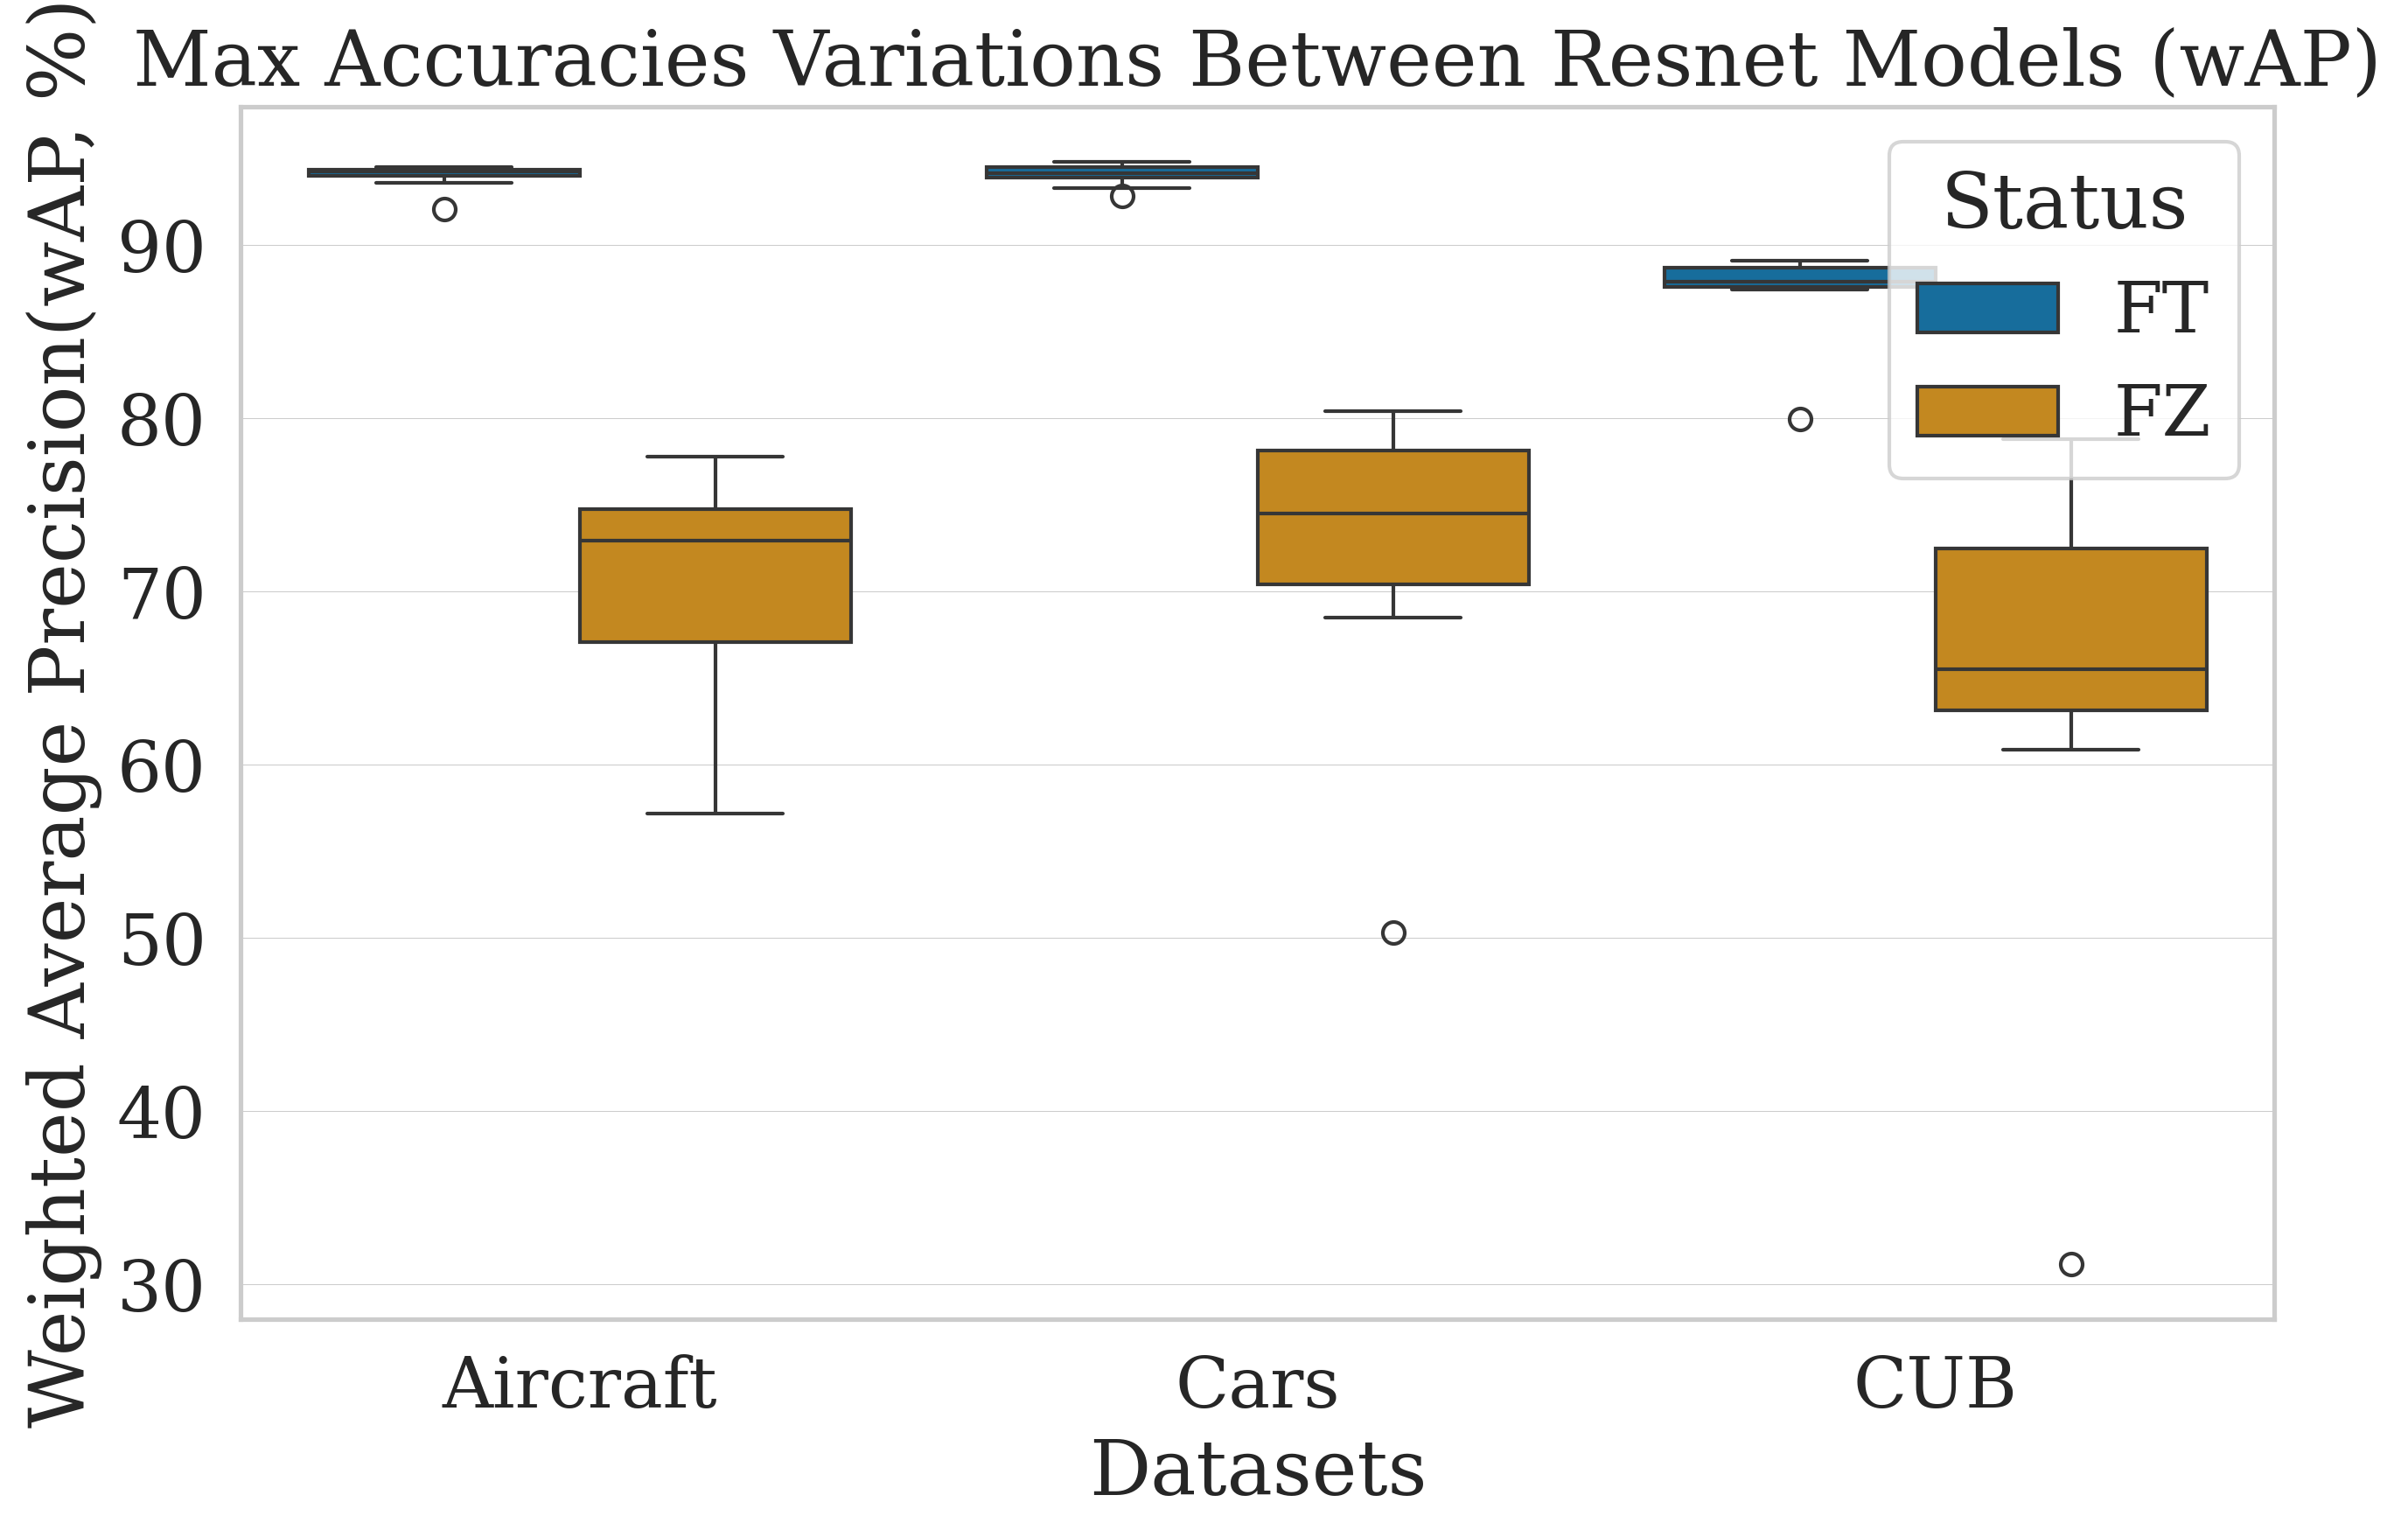
\includegraphics[width=\linewidth]{figures/imgs/performance_left.png}
        \label{fig:resnet_perf}
    \end{minipage}
    \hspace{0.01\linewidth} % Reduce spacing
    \begin{minipage}{0.41\linewidth}
        \centering
        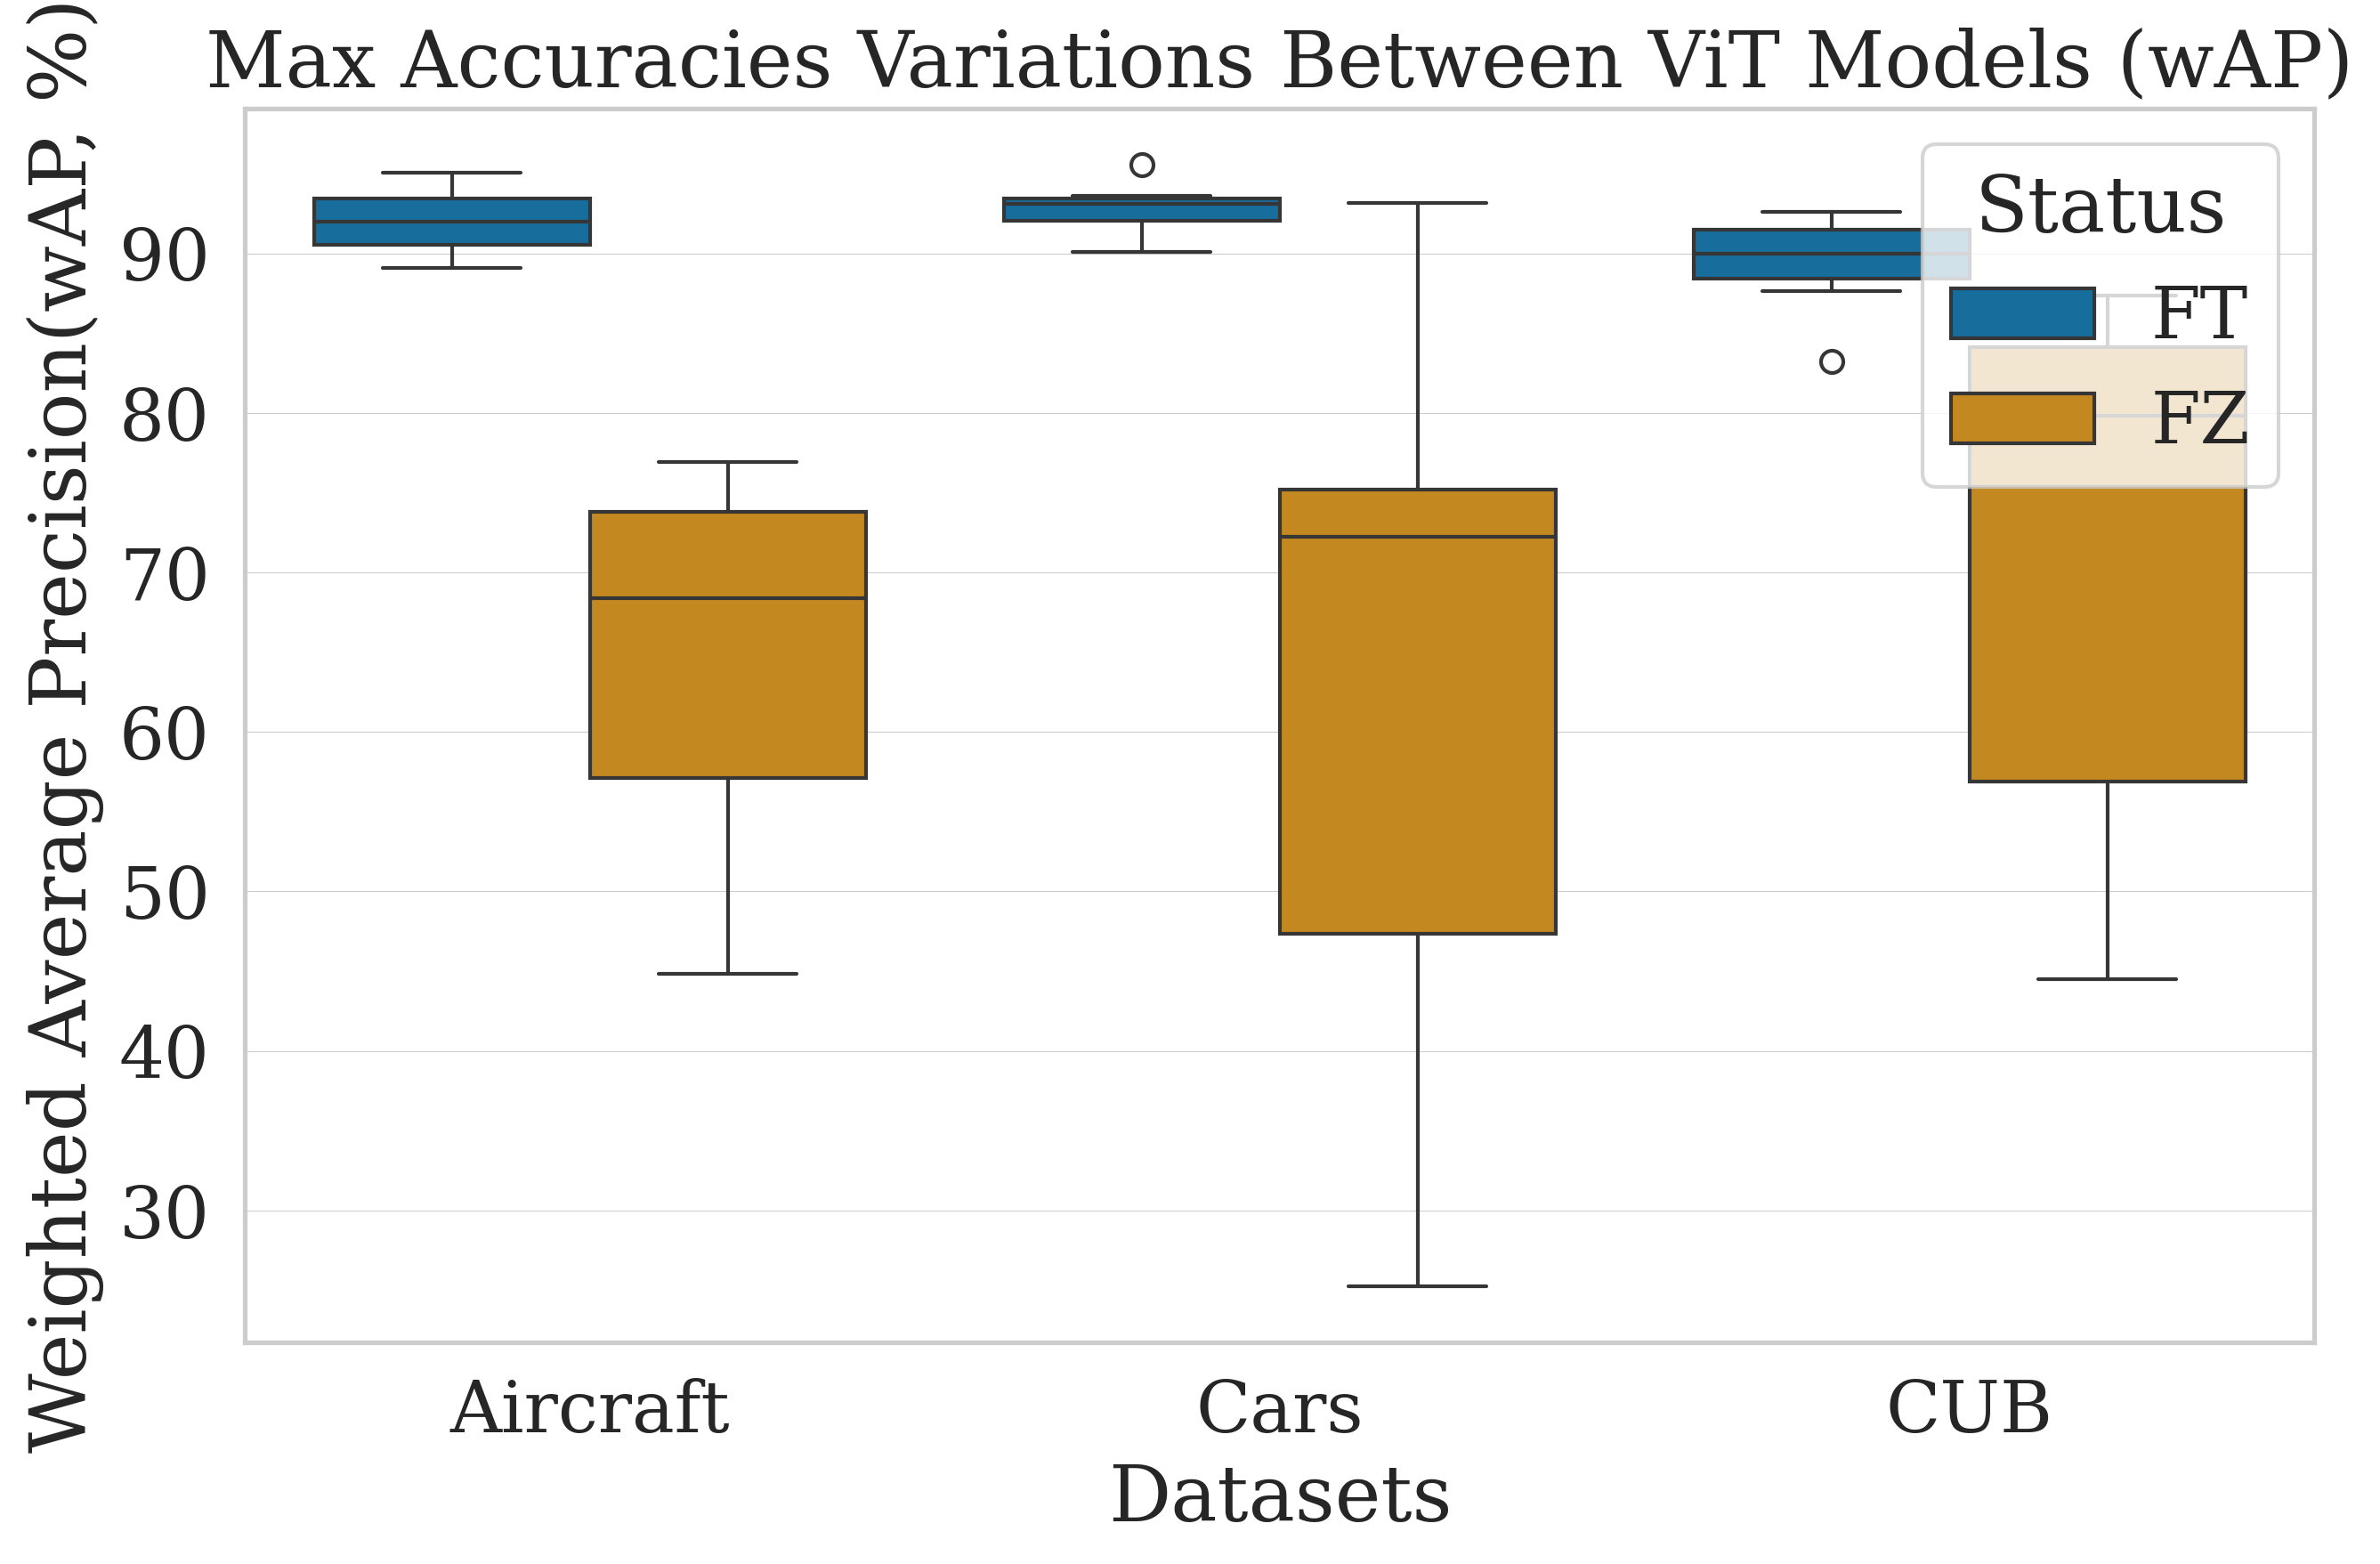
\includegraphics[width=\linewidth]{figures/imgs/performance_right.png}
        \label{fig:vit_perf}
    \end{minipage}
    \vspace{-0.55cm}
    \caption{Performance variability across backbone types and training modes. We compare fine-tuned (FT) and frozen (FZ) variants of ResNet (left) and ViT (right) models across hierarchical FGIR benchmarks.}
    \label{fig:performance}
\end{figure*}

\subsection{Hyperparameters and Optimization}
We conducted our experiments using the following set of hyperparameters and training configurations:
\begin{itemize} [topsep=3pt, itemsep=2pt, parsep=1pt]
    \item SGD: \{0.3, 0.1, 0.03, 0.01, 0.003\}
    \item AdamW: \{0.005, 0.001, 0.0005, 0.0001, 0.00005, 0.00001, 0.000005\}
\end{itemize}
Weight decay is set to 0 (SGD) and 0.05 (AdamW).

\vspace{1em}

We trained the models for a total of 200 epochs with batch size of 8 images. We used Cosine Anneal Scheduler and used Mixed Precision Training. Images were resized to a square shape of 550x550 pixels. During training, random cropping was applied to generate patches of size 448x448 pixels, while during inference, the center area was cropped to the same size (Random Cropping), a horizontal flip was applied during training to augment the dataset.

\section{RESULTS}
\subsection{Impact of Backbone and Pretraining}
\subsubsection{Choice of backbone and hyperparameter do matter}
The choice of backbone and hyperparameter configuration has a significant impact on hierarchical FGIR performance. As shown in Table ~\ref{tab:overallperf}, applying the pipeline from Chang et al.~\cite{chang_your_2021} , and \textbf{through careful selection of backbones and hyperparameters}, we were able to achieve \textbf{state-of-the-art accuracy on both ResNet and ViT models} even \textbf{with older architecture}. This shows the importance of backbone selection and hyperparameter tuning in optimizing hierarchical FGIR performance.

\vspace{-0.2cm}
\subsubsection{Distinct differences between ResNet and ViT models}
The performance of both ResNet and ViT models shows distinct patterns. In general, \textbf{ResNet models are more robust than ViT models regardless of pretrainings and hyperparameters}, seen in fig. ~\ref{fig:performance}. The \textbf{gap between worst fine-tuned and best frozen is small}, especially for ViT models, this gap is worth noting as \textbf{frozen settings} only \textbf{train less than 0.05\% of the trainable parameters}.

\vspace{-0.2cm}
\subsubsection{Backbone Choice Can Yield SoTA or Suboptimal Results}
Figure~\ref{fig:best_a_worst} further illustrates the importance of backbone selection. For ResNets, top-performing models (e.g., MoCoV3) achieve near identical accuracy across datasets, MoCov3 obtains 94\% wAP in Aircraft, while worst performing Resnet Spark 92\% wAP. In contrast, ViT models show greater spread: SigLIP-v2 leads on Aircraft 94\% wAP and Cars 95\% wAP, while base ViT outperforms others on CUB 91\% wAP. Worst ViT model is obtained by DINO with 87\% wAP on Aircraft and 89\% on Cars. These findings underscore that backbone selection, particularly for ViTs, can lead to either \textbf{SoTA performance or significantly degraded results}.

\begin{figure*}[!htb]
    \centering
    \begin{minipage}{0.42\linewidth}
        \centering
        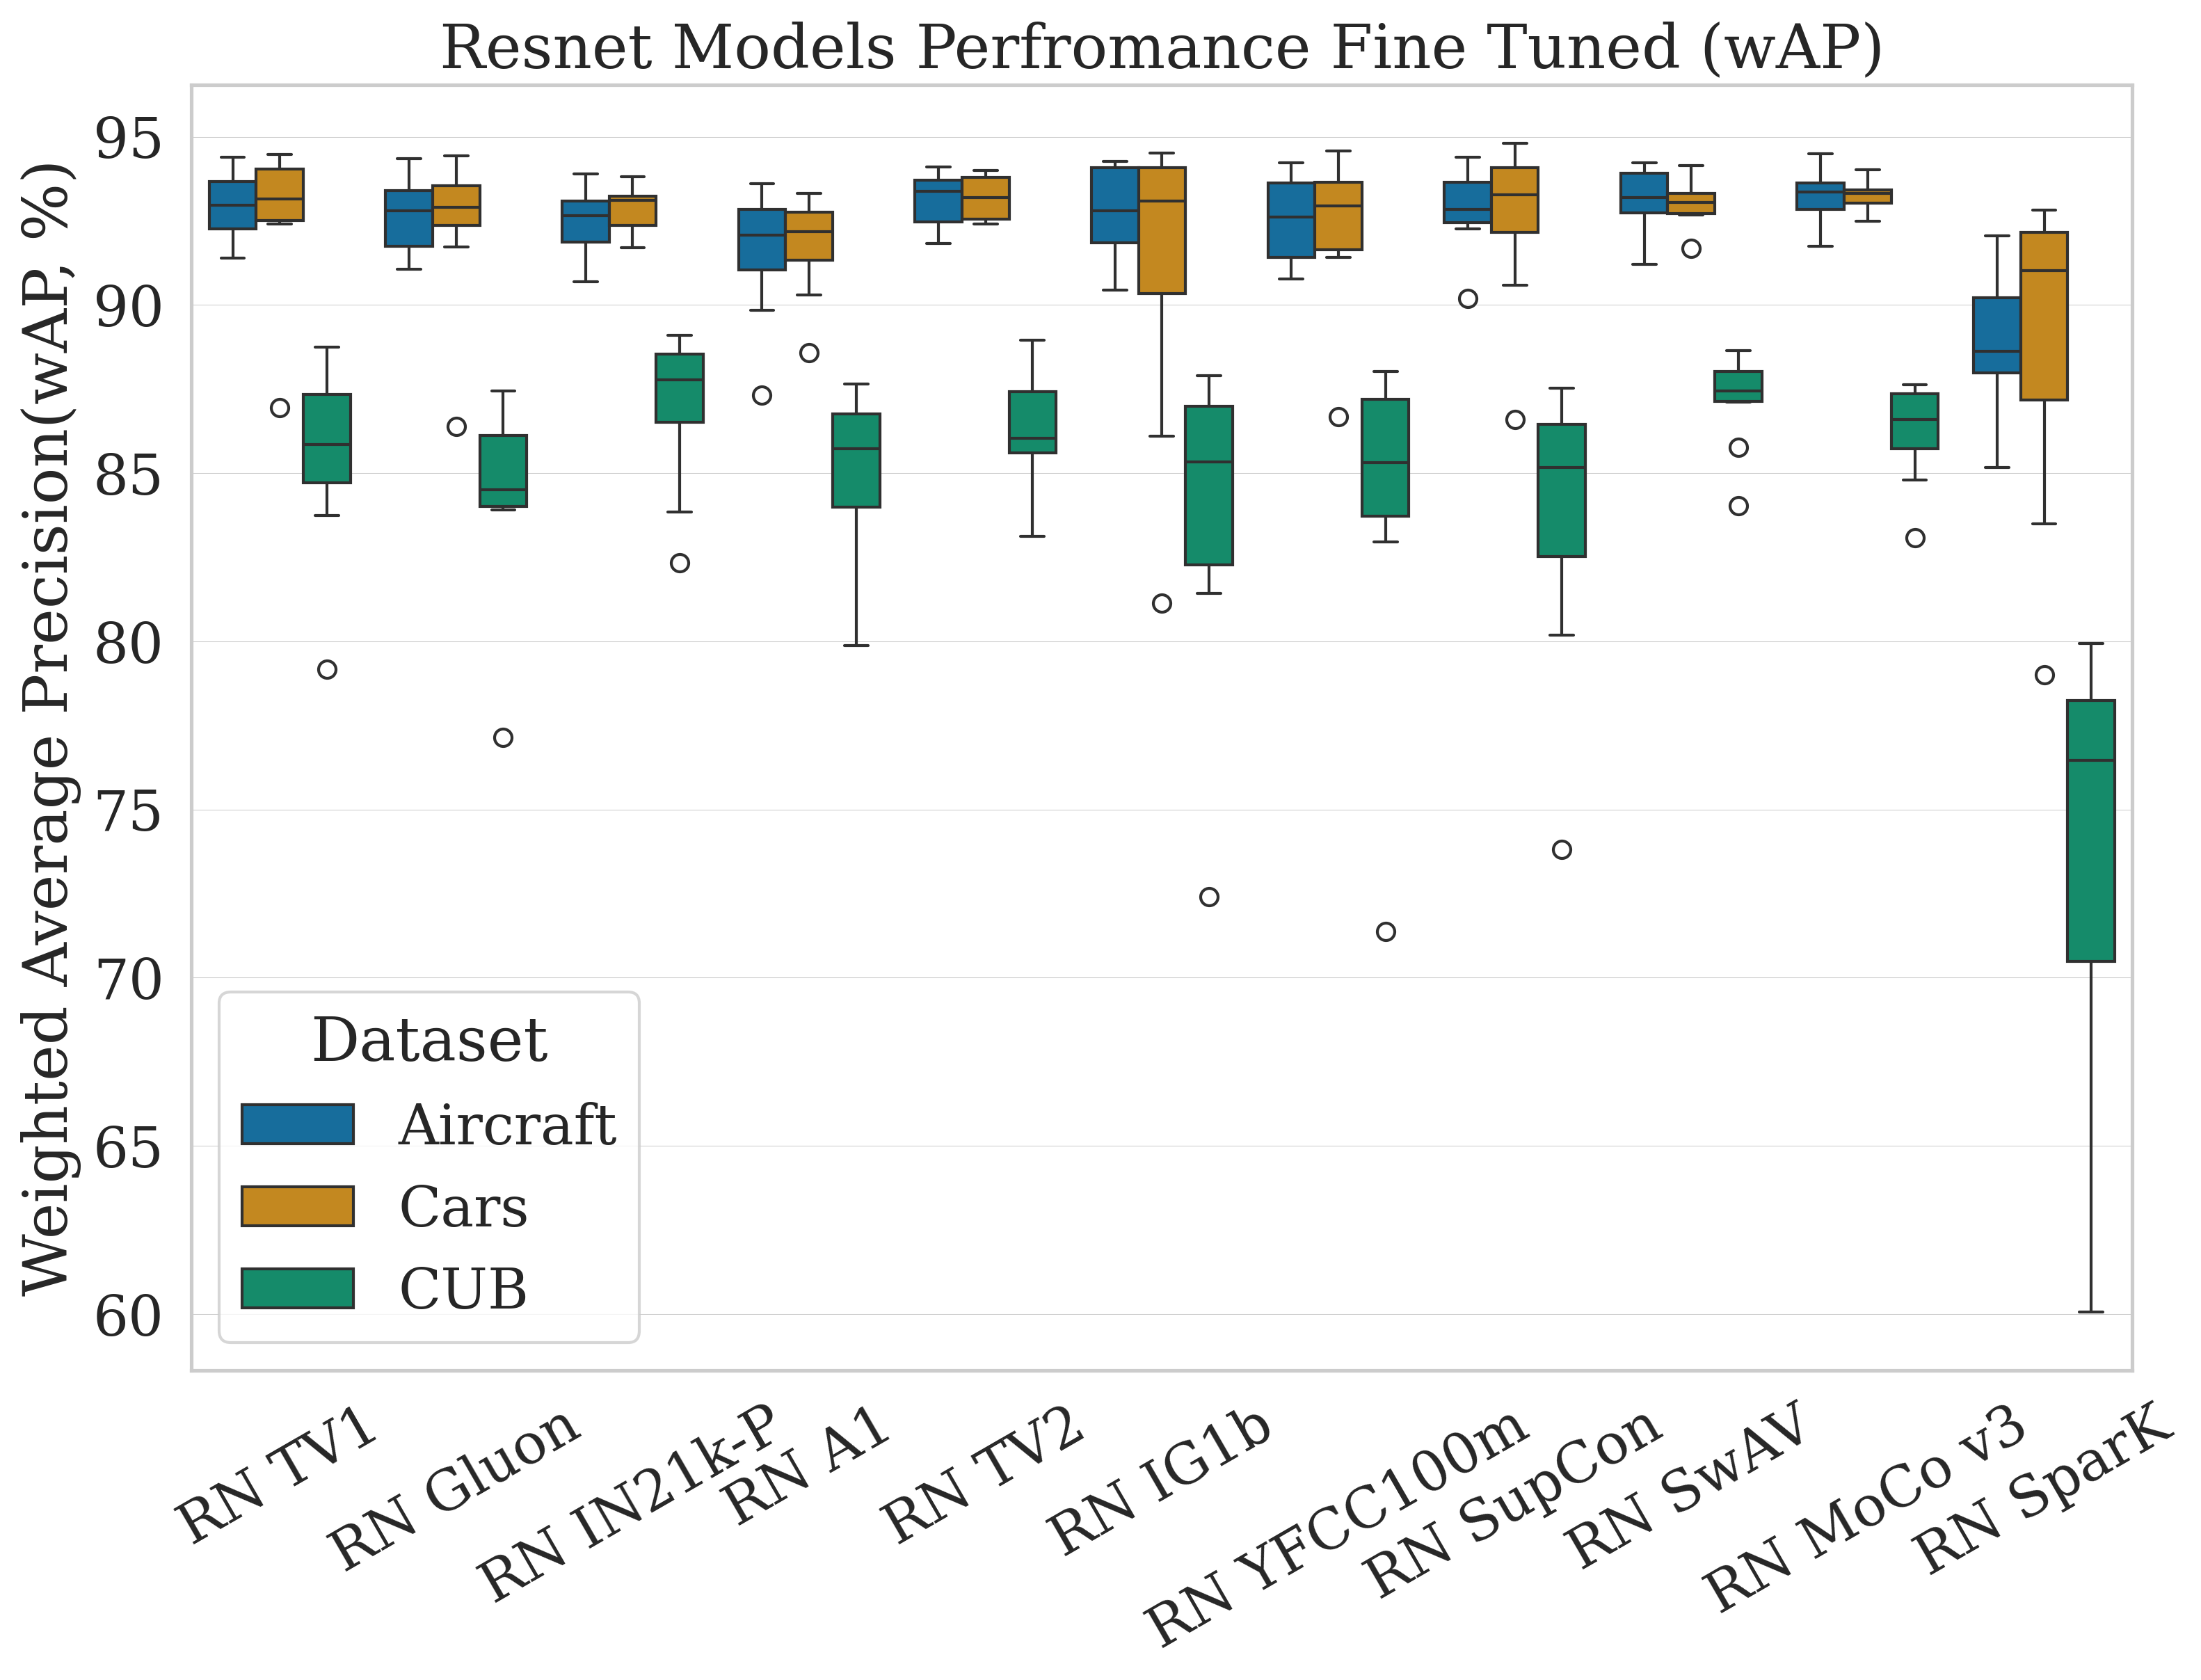
\includegraphics[width=\linewidth]{figures/imgs/rn_ft.png}
        \label{fig:rn_ft}
    \end{minipage}
    \hspace{0.01\linewidth} % Reduce spacing
    \begin{minipage}{0.42\linewidth}
        \centering
        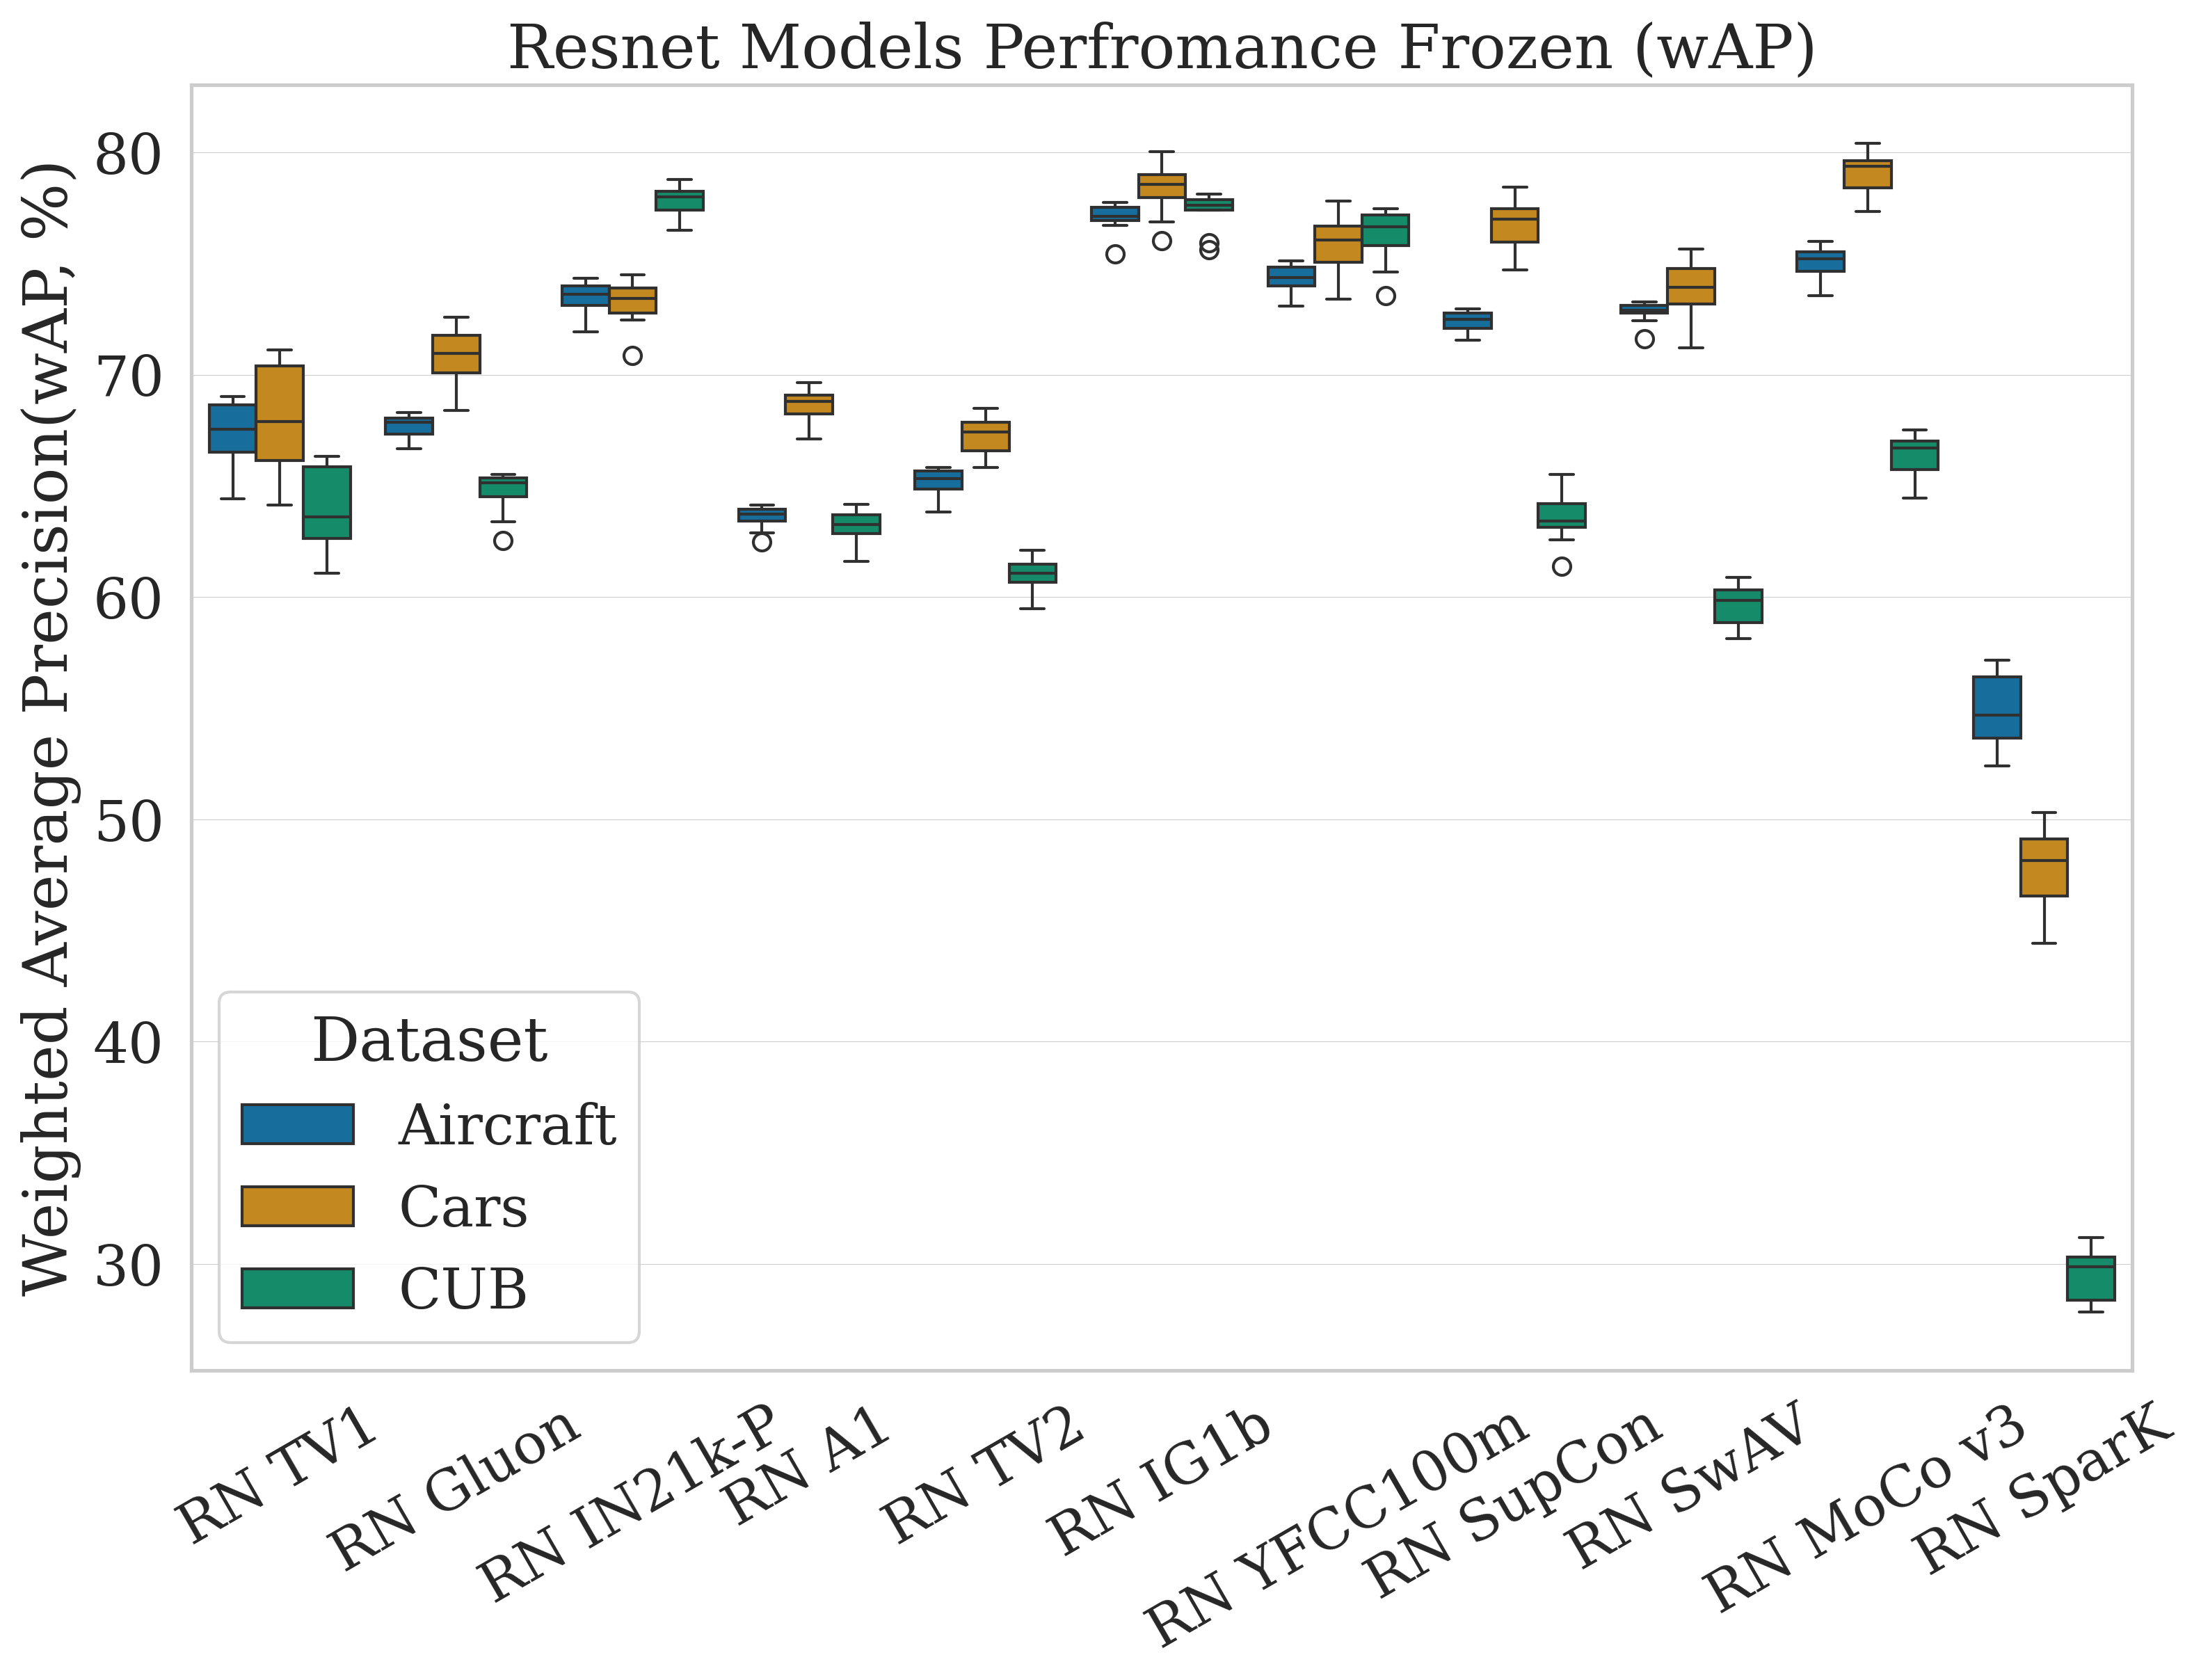
\includegraphics[width=\linewidth]{figures/imgs/rn_fz.png}
        \label{fig:rn_fz}
    \end{minipage}

    \centering
    \begin{minipage}{0.42\linewidth}
        \centering
        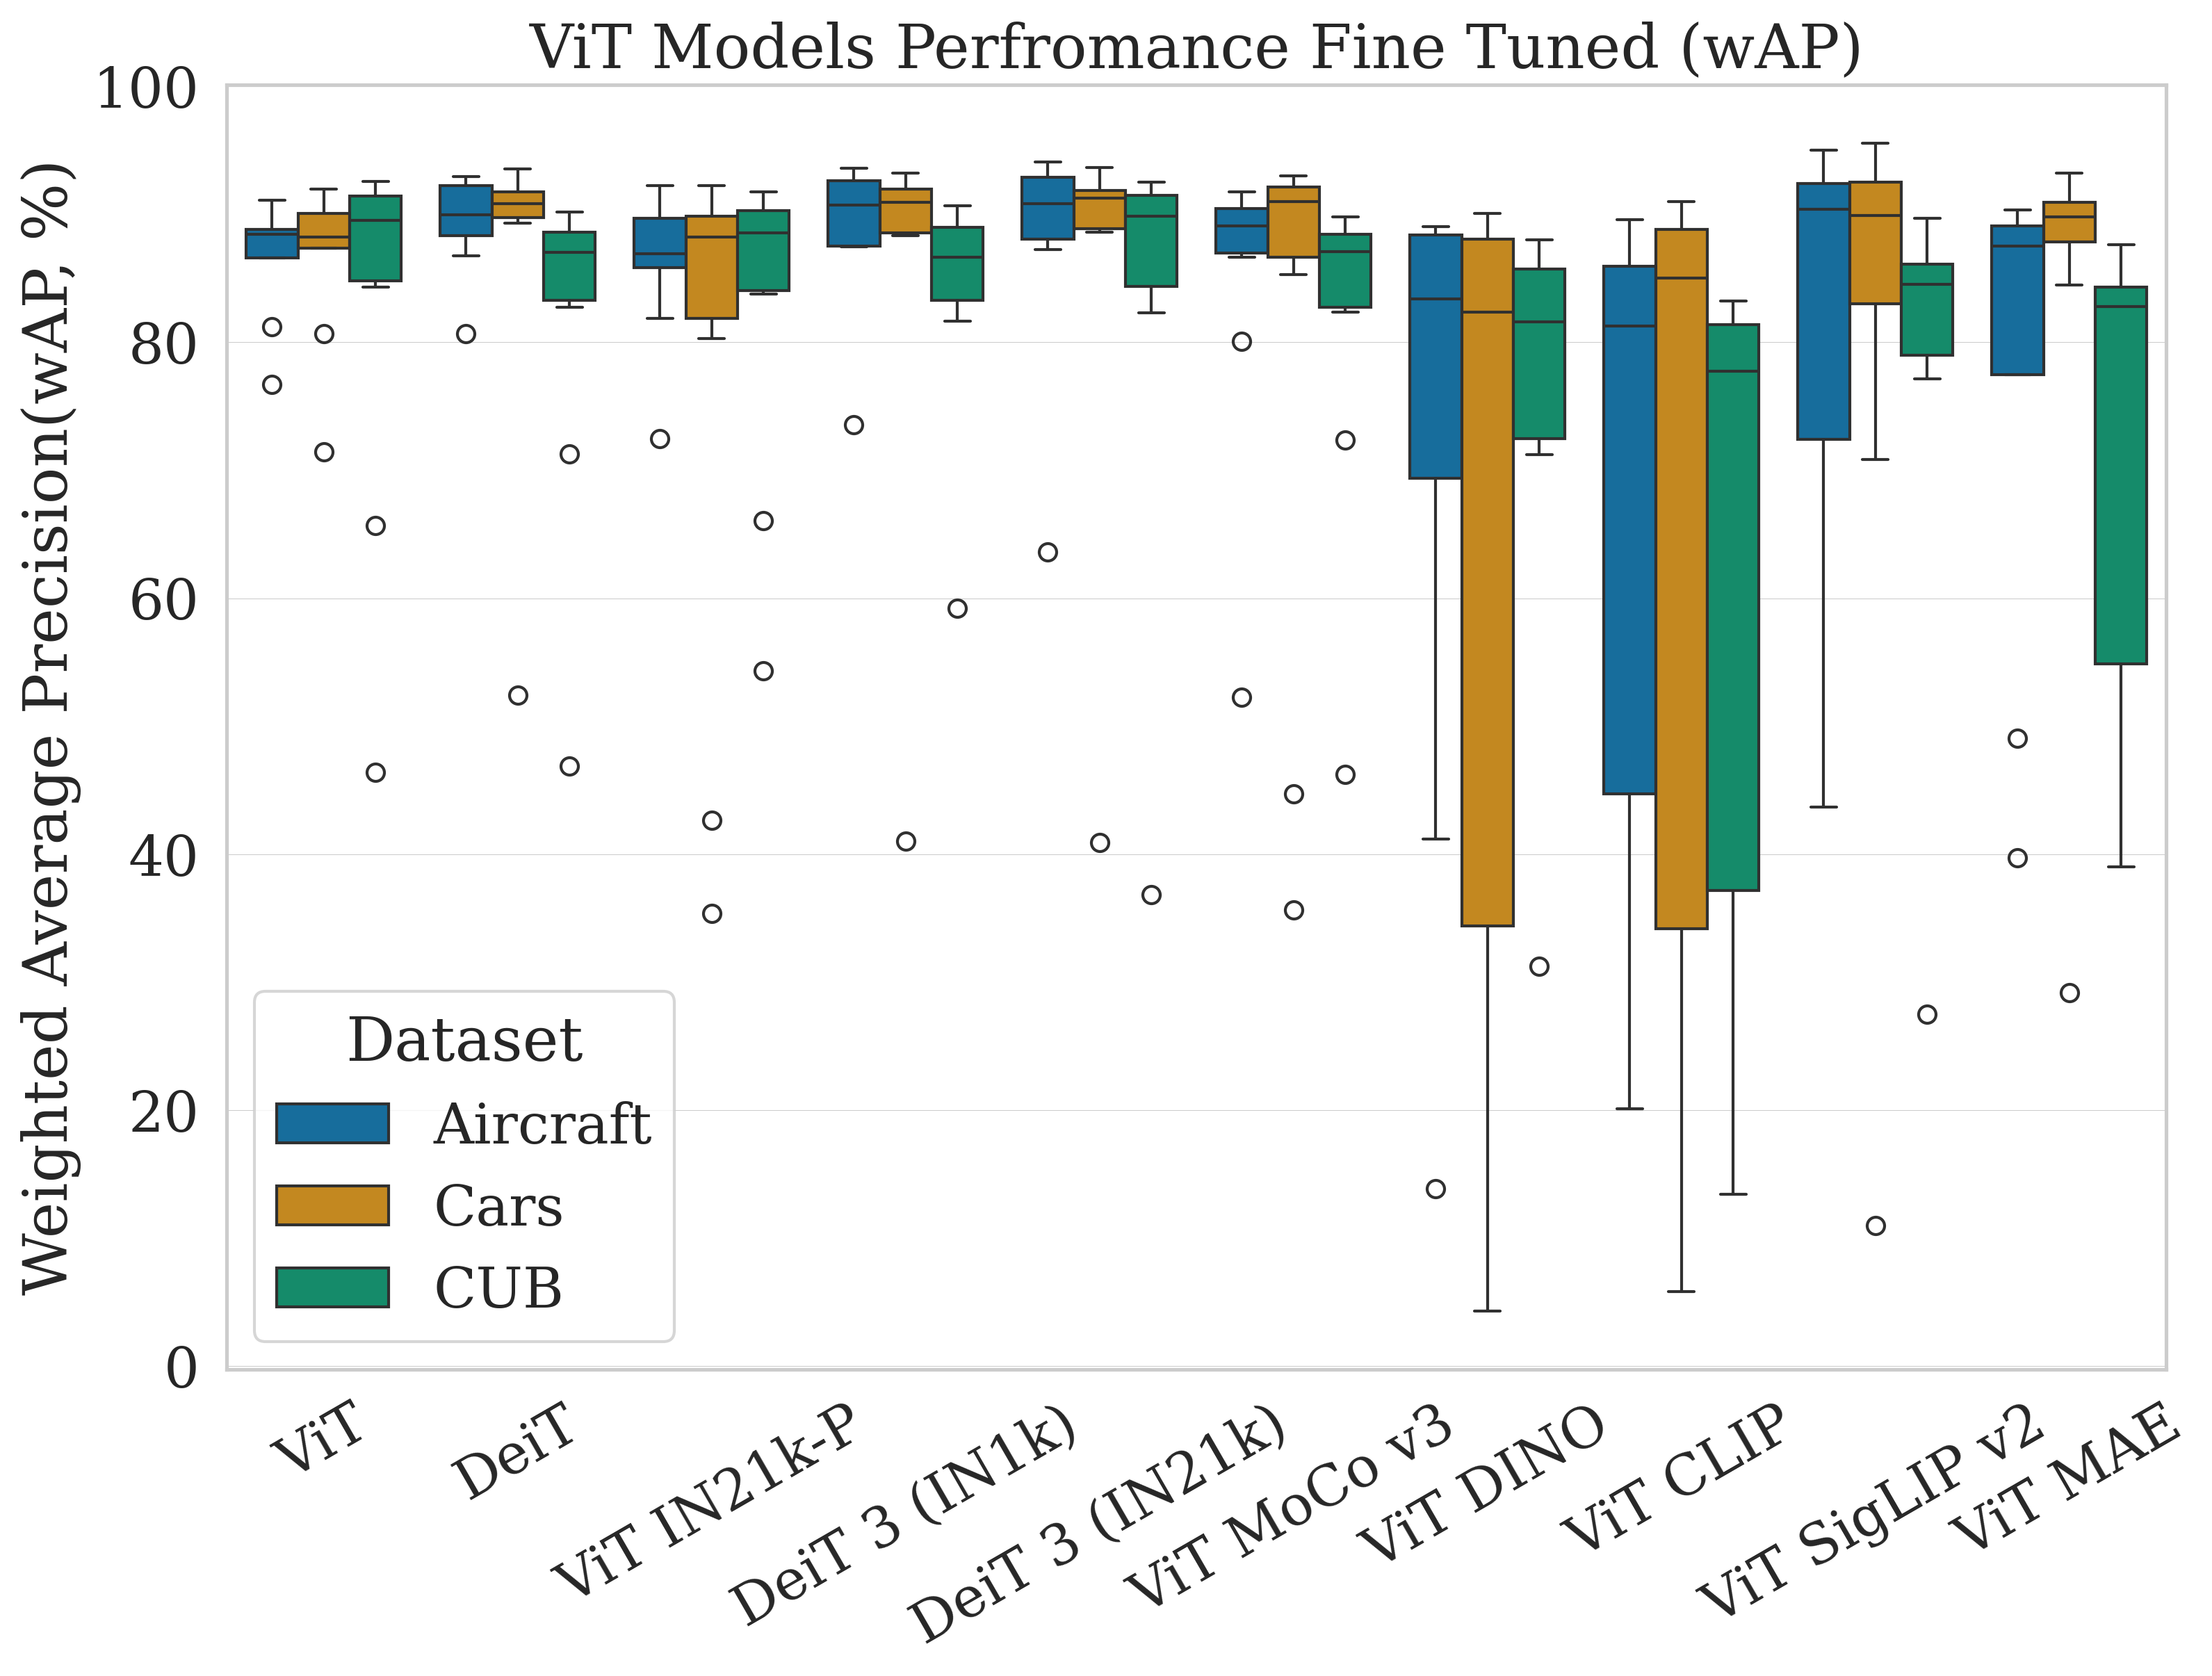
\includegraphics[width=\linewidth]{figures/imgs/vit_ft.png}
        \label{fig:vit_ft}
    \end{minipage}
    \hspace{0.01\linewidth} % Reduce spacing
    \begin{minipage}{0.42\linewidth}
        \centering
        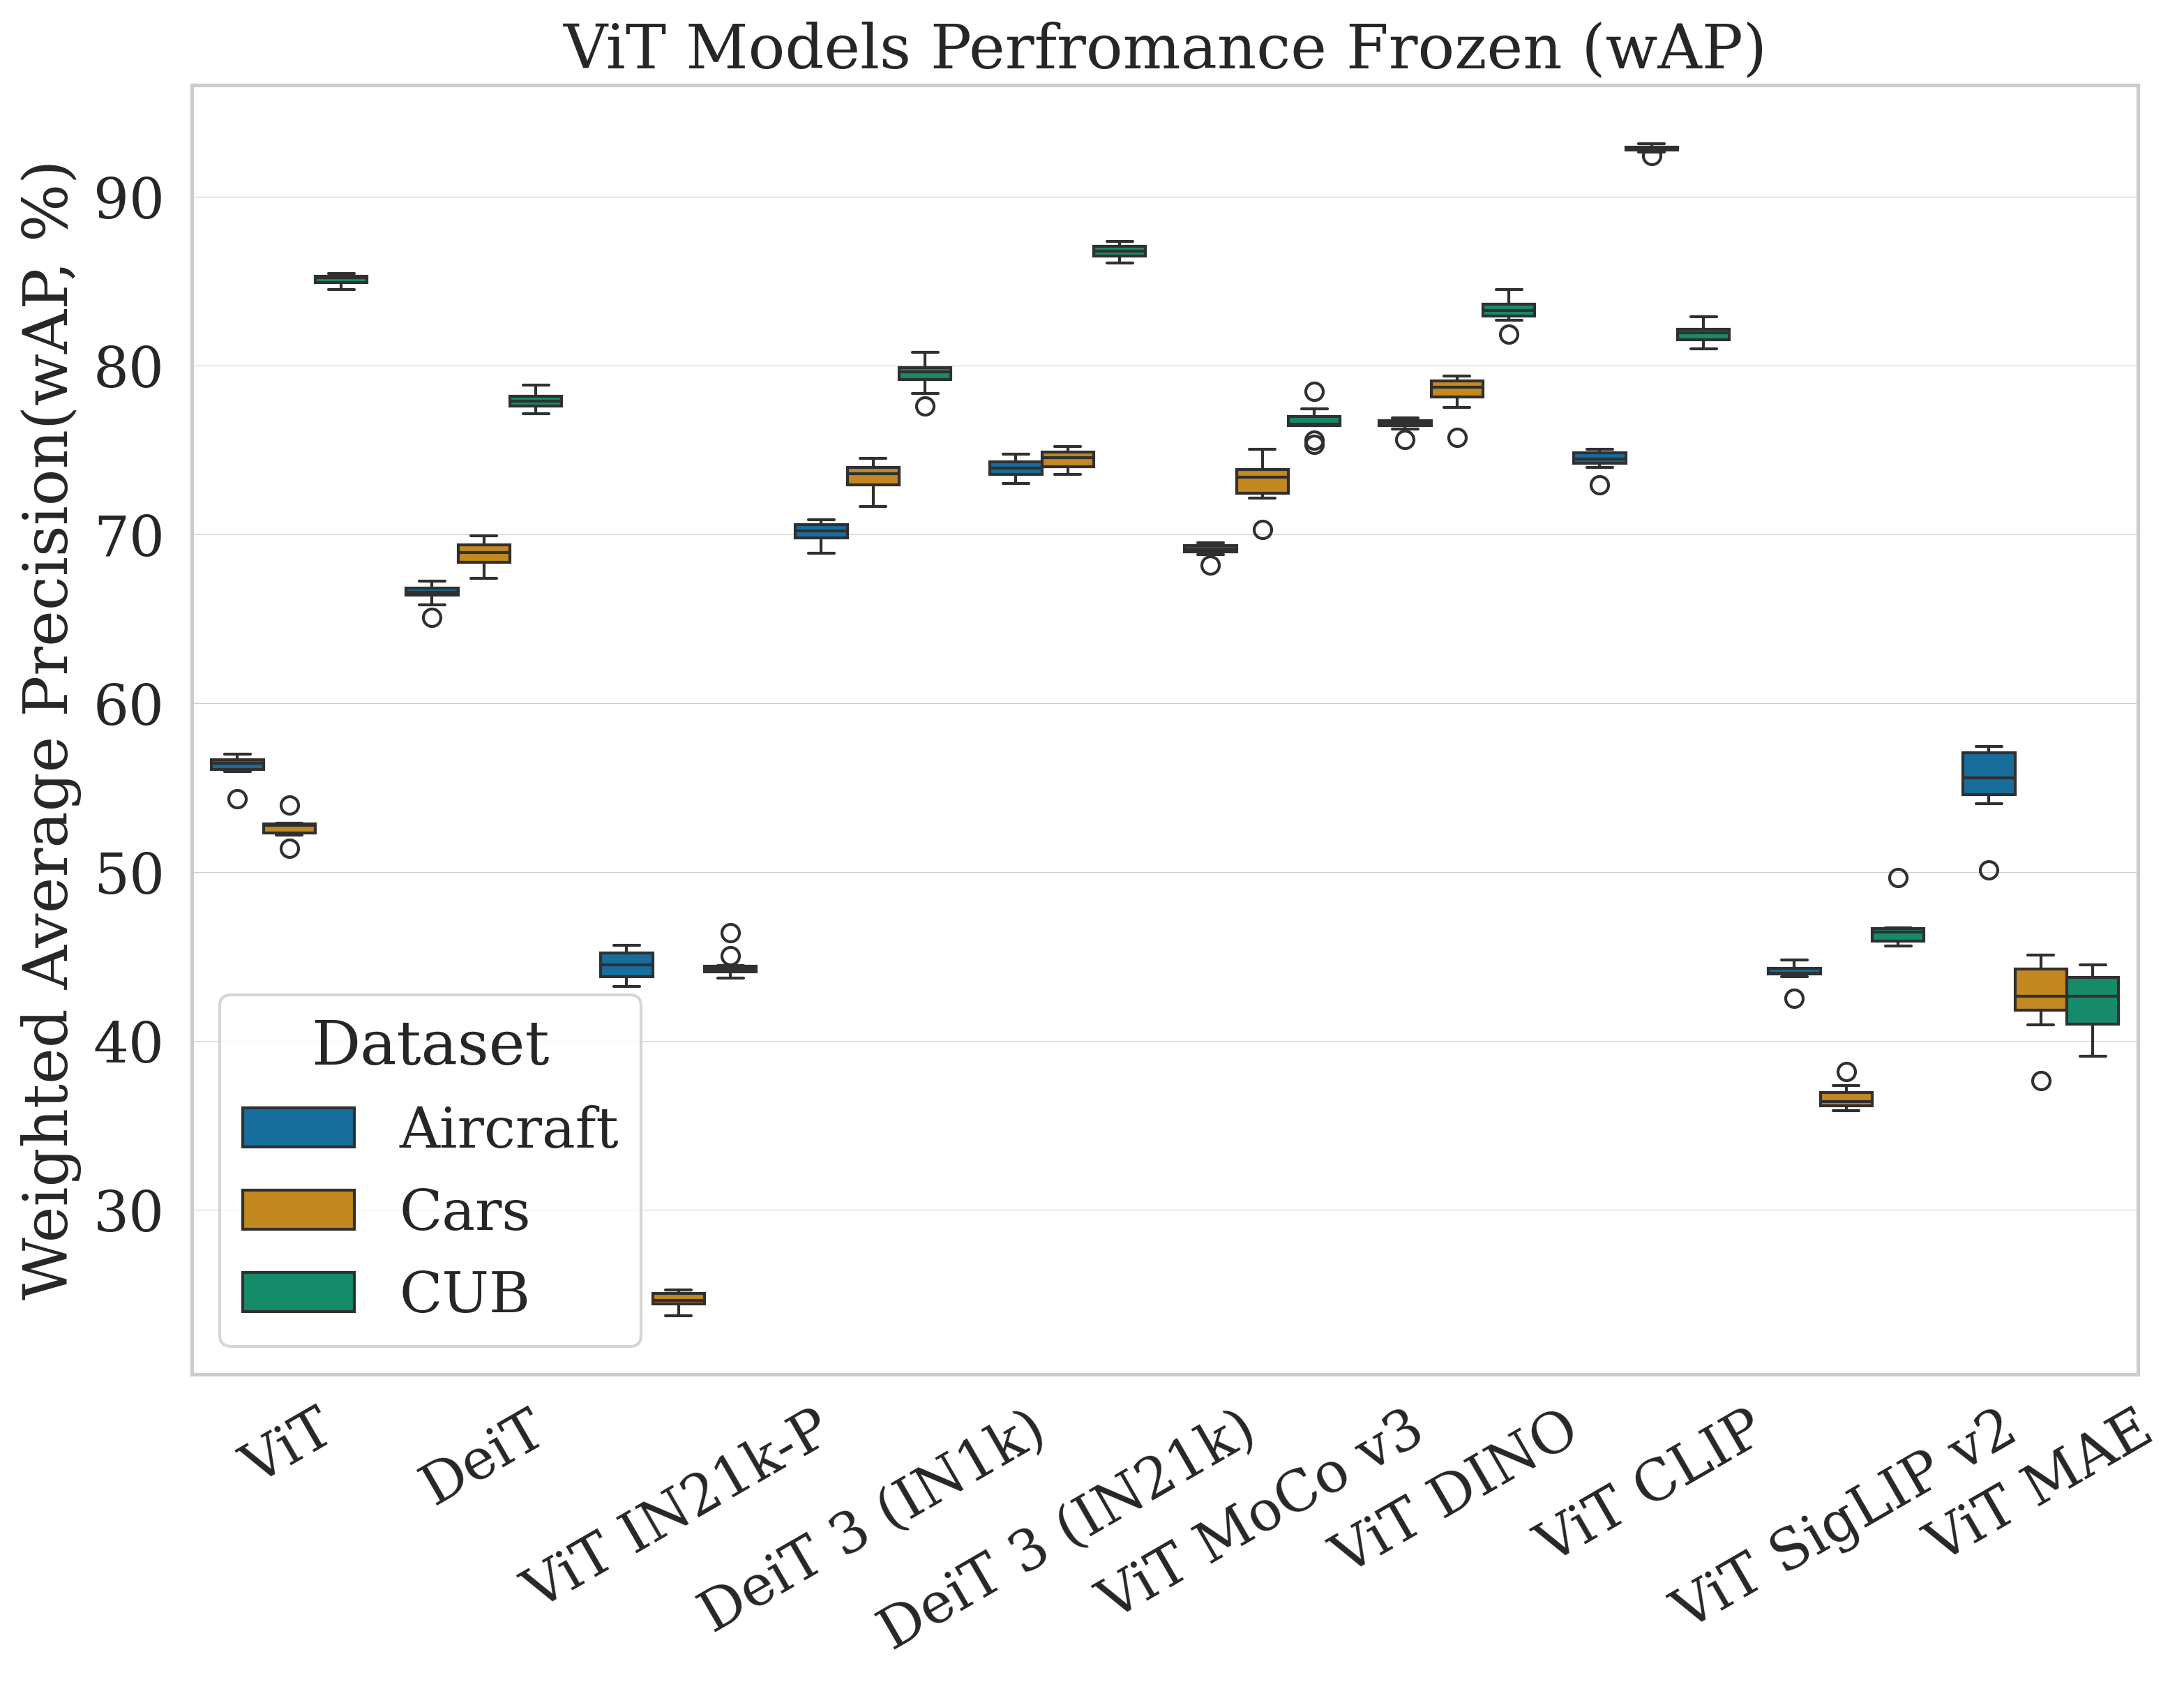
\includegraphics[width=\linewidth]{figures/imgs/vit_fz.png}
        \label{fig:vit_fz}
    \end{minipage}
    \vspace{-0.55cm}
    \caption{Backbone performance across training regimes. We compare ResNet (top) and ViT (bottom) models under fine-tuned (FT, left) and frozen (FZ, right) settings. Each plot shows the wAP performance distribution across models with different pretraining strategies.}
    \label{fig:four_plot}
\end{figure*}

\vspace{-0.2cm}
\subsection{Impact of Hyperparameters}
\subsubsection{Distribution of Results}
In figure~\ref{fig:four_plot}, Under \textbf{fine-tuned settings}, \textbf{ResNet models} pretrained via \textbf{discriminative models} (e.g., MoCoV3, SwAV) achieve the highest accuracy and lowest variance. Under \textbf{frozen setting}, \textbf{semi-supervised ResNet models} (e.g., IG1b, YFCC300m) and the IN21K-pretrained model outperform others, suggesting that pretraining dataset significantly influences performance under frozen settings.

For ViT models, Fine-Tuned Fully Supervised models such as
base ViT, DeiT, and DeiT3 demonstrate both high mean accuracy and
low standard deviation in fine-tuned settings. In the Frozen settings, Discriminative models like MoCoV3 and CLIP achieve the best performance.

\vspace{-0.2cm}
\subsubsection{Discriminative models perform best for both training settings}
\textbf{Discriminative models} (e.g. MoCoV3, SwAV) obtains the best performance for both training settings, as observed in Fig.~\ref{fig:four_plot}. Among the discriminative approaches, \textbf{contrastive methods outperform non-contrastive alternatives} (e.g. ViT DINO). This highlights the effectiveness of contrastive learning as a pretraining strategy for models deployed in structured, fine-grained classification pipelines. Discriminative models, trained via contrastive or predictive learning, is the best approach to tackle the core challenge of FGIR.

\vspace{-0.2cm}
\subsubsection{Size of pretraining Dataset influences frozen performance}
\textbf{Semi-Supervised models} (IG1b, YFCC300m) and the \textbf{IN21K-P model achieve the best results} for ResNet \textbf{under the Frozen setting}. A common feature among these 3 models is that they are \textbf{pretrained on larger datasets, IG1b, YFCC300m, In21k accordingly}. For ViT models, where base ViT, DeiT (IN21K), and CLIP models achieve high accuracy, particularly on the CUB dataset. These models share the characteristic of pretrained on larger datasets, In21k, LAION5b accordingly, as observed in figure ~\ref{fig:four_plot}.

\vspace{-0.2cm}
\subsubsection{Analysis on undeperforming models}
\textbf{Generative models} (e.g SparK, MAE) and DINO underperforms for both ResNet and ViT backbones, as observed in Fig. ~\ref{fig:four_plot}. These models employ distinct pretraining strategies, masked image reconstruction for generative models and self-distillation for DINO, which fails to capture local features. This indicates that \textbf{this strategy is not well suited for frozen settings in hierarchical FGIR tasks}.

% \vspace{-0.2cm}
% \subsubsection{CLIP model does better on frozen than fine-tuning settings}
% In contrast, the \textbf{CLIP model performs better under frozen settings} than in fine-tuning settings. CLIP employs a unique classification approach known as zero-shot classification, which compares image embeddings with text embeddings to make predictions. However, in our experiment, we \textbf{did not utilize the zero-shot classification head}, making the fine-tuning of the weights ineffective. This redundancy led to the model underperforming in the fine-tuning setting. (Figure ~\ref{fig:four_plot})

\vspace{-0.2cm}
\subsubsection{Resnet models do better on Aircraft, Cars, but ViT models
do better on CUB}
In figure (Fig. ~\ref{fig:best_a_worst}) and (Fig. ~\ref{fig:four_plot})ResNet models perform better on Aircraft and Cars, while ViT models perform better on CUB. This aligns with Ye et al. \cite{ye_image_2024}, which suggests that the nature of object shapes plays a role in model effectiveness. ViT’s self-attention mechanism enables global context modeling from early layers, making it more suited for datasets with high shape variability (e.g. birds). In contrast, CNNs like ResNet incorporate inductive biases, this introduces locality and translation invariance, which favor texture-sensitive data, especially for objects with relatively rigid and static structures (e.g. vehicles).  Moreover, ViT has bigger image patches than Resnet. This bigger patch size might have enabled ViT to capture better global features. 

Additionally, it is worth noting that ImageNet contains a substantial number of bird-related images, which may have contributed to a performance boost for ViT models on the CUB dataset. This supports the idea that the performance of these architectures varies depending on the type of objects in the dataset and the pretraining data they are exposed to.

\begin{figure*}[ht]
    \centering
    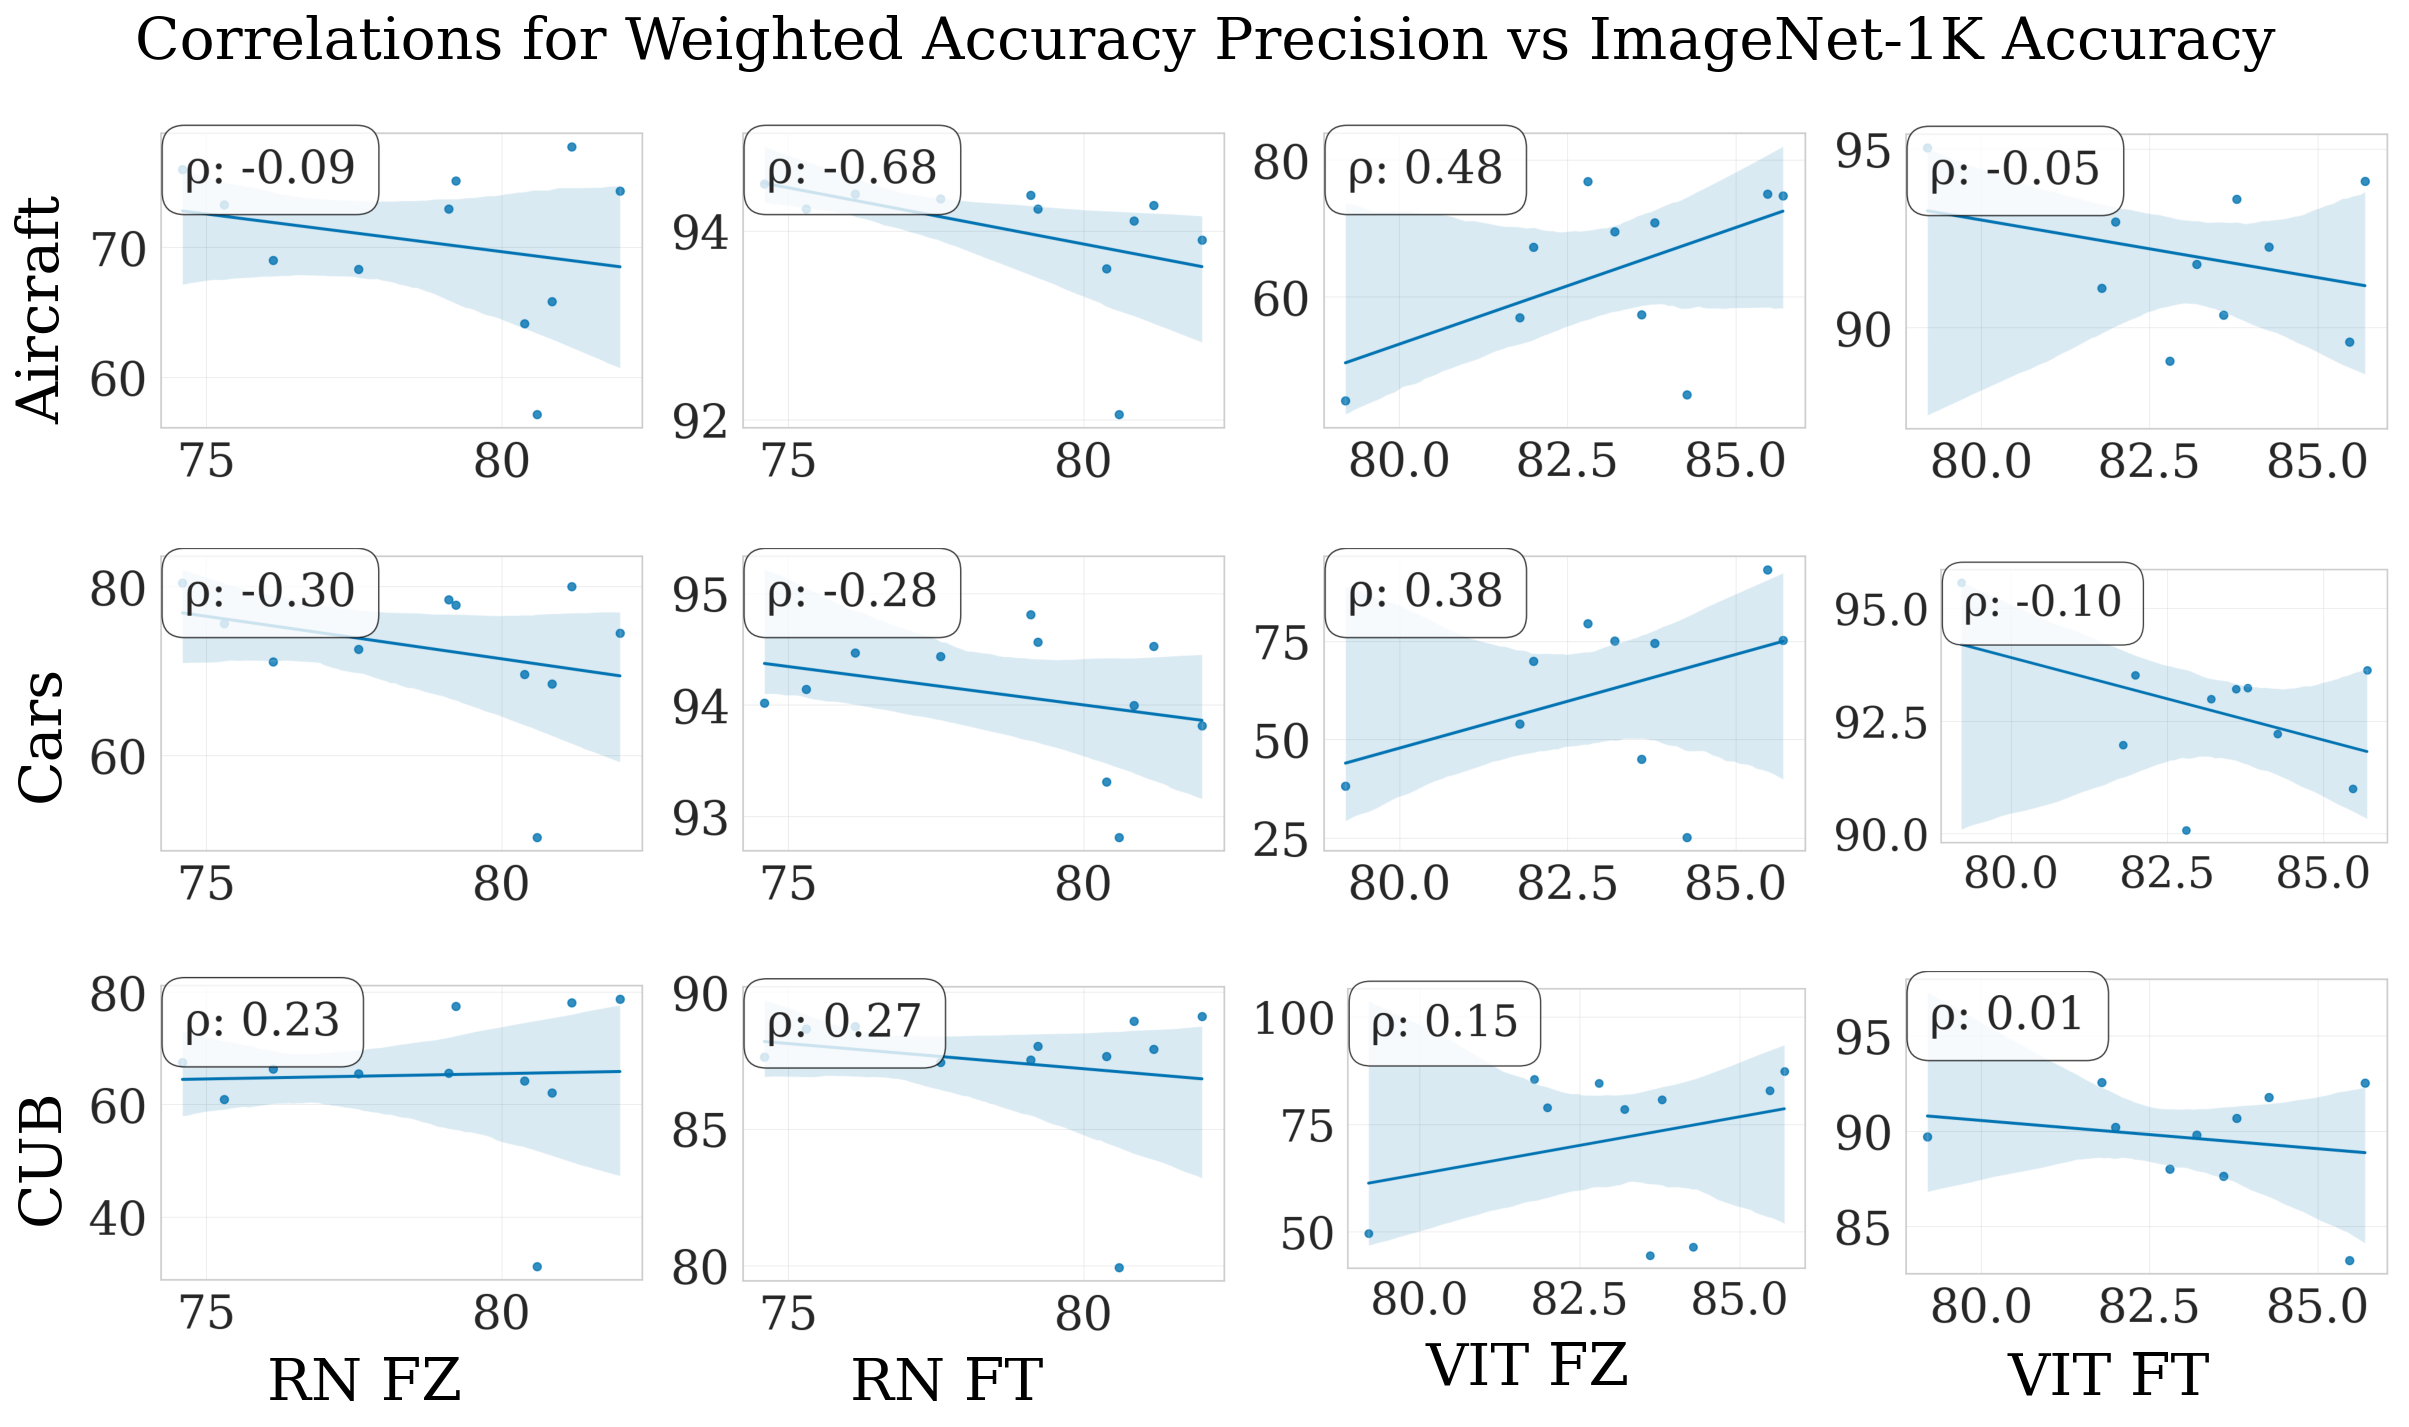
\includegraphics[width=0.6\linewidth]{figures/imgs/example_metric.png}
    \caption{Correlation between Imagenet-1k accuracy and wAP. Its correlation with downstream performance is weak, reflecting a broader trend observed across all tested metrics.} 
    \label{fig:example_metric}
\end{figure*}

\subsection{Metric Correlation}
Across all models, datasets, and evaluation targets, most transferability metrics—such as CKA, ImageNet-1k accuracy, and CIS~\cite{kornblith_better_2019, nayman_diverse_2022} exhibit weak or inconsistent correlations with performance. As an illustrative example, Fig.~\ref{fig:example_metric} shows the correlation between a representative metric and Top-1 accuracy, highlighting the general trend: \textbf{no single metric reliably predicts downstream performance in the hierarchical FGIR setting}. While these metrics have demonstrated efficiency in standard transfer learning tasks, \textbf{they fail to generalize to hierarchical classification}. We attribute this to the added \textbf{complexity introduced} by the \textbf{hierarchical method}. This reveals a gap between general transferability and hierarchical recognition, highlighting the need for predictive metrics tailored for hierarchical FGIR.

% \vspace{-0.15cm}
% \subsubsection{MSC and CIS(Spectral) Show Strong Correlation with Accuracy in Frozen ViT Models}
% We observe that both \textbf{MSC} and \textbf{CIS (Spectral)} exhibit moderate to strong positive Spearman correlations ($\rho$) with \textbf{Top-1 accuracy} in frozen ViT models. For MSC, the highest correlation is observed on CUB-200 ($\rho = 0.8$), followed by Stanford Cars ($\rho = 0.6$), and FGVC Aircraft ($\rho = 0.3$). Similarly, CIS(Spectral) achieves its strongest correlation on CUB $\rho = 0.8$, with Cars and Aircraft following at $\rho = 0.6$ and $\rho = 0.5$, respectively. These results suggest that both local similarity (MSC) and spectral diversity (CIS) are predictive of performance in frozen ViTs. Notably, the strong performance of CIS(Spectral) supports findings from Nayman et al.~\cite{nayman_diverse_2022}, which emphasize the efficacy of spectral diversity in frozen settings, though we observe this primarily for ViT architectures.

% \begin{figure}[ht]
%     \centering
%     \includegraphics[width=\linewidth]{figures/imgs/high_mean.png}
%     \caption{CKA(High Layers) correlation, see VIT+FT} 
%     \label{fig:high_mean}
%     \vspace{-0.3cm}
% \end{figure}

% \vspace{-0.2cm}
% \subsubsection{CKA(High Layers) Show Strong Correlation with Accuracy in Fine-tuned ViT Models}
% We observe that \textbf{CKA (High Layers)} exhibits moderate to strong positive correlation with \textbf{Top-1 accuracy} in fine-tuned ViT models. On CUB, it achieves the strongest correlation $r = -0.7$, while on Cars and Aircraft, Spearman correlations are stronger with consistently achieving around $rho = -0.5$. This pattern suggests that similarity in deeper layers, measured through representational alignment, is indicative of effective fine-tuning in ViT architectures. These findings align with the hypothesis that high-level feature consistency plays a crucial role in adapting transformers for fine-grained tasks under end-to-end training regimes.

% \begin{figure}[ht]
%     \centering
%     \includegraphics[width=\linewidth]{figures/imgs/low_mean.png}
%     \caption{CKA(Low Layers) correlation, see RN+FZ} 
%     \label{fig:low_layer}
%     \vspace{-0.3cm}
% \end{figure}

% \vspace{-0.2cm}
% \subsubsection{CKA(Low Layers) Show Strong Correlation with Accuracy in Frozen Resnet Models}
% For frozen ResNet backbones, \textbf{CKA (Low Layers)} demonstrates strong positive correlation with \textbf{Top-1 accuracy} in frozen Resnet models. On CUB, it achieves the strongest correlations of $r = 0.74$, followed by $r = 0.66$ on FGVC Aircraft, and $r = 0.23$ on Stanford Cars. These observations suggest that representational similarity in early layers is a key indicator of effective feature reuse in CNN-based architectures when the backbone remains frozen. This finding reinforces the importance of low-level feature quality in scenarios where most model weights are fixed during training.

% \begin{figure}[ht]
%     \centering
%     \includegraphics[width=\linewidth]{figures/imgs/l2_norm.png}
%     \caption{L2 norm correlation, see RN+FZ} 
%     \label{fig:l2_norm}
%     \vspace{-0.3cm}
% \end{figure}

% \vspace{-0.2cm}
% \subsubsection{L2 Norm Show Strong Correlation with Accuracy in Fine-tuned Resnet Models}
% We find that the \textbf{L2 norm} exhibits moderate to strong negative correlation with \textbf{Top-1 accuracy} in fine-tuned ResNet models. The highest negative Spearman correlation is observed on Stanford Cars $\rho = -0.87$, followed by FGVC Aircraft($\rho = -0.7$, and CUB $\rho = -0.5$. These results imply that larger feature magnitudes are associated with degraded performance in fine-tuned settings, possibly reflecting instability or overconfidence in the learned representations. This trend appears specific to convolutional backbones under fine-tuning, and may signal the need for additional normalization or regularization strategies in such regimes.

% \vspace{-0.2cm}
% \subsubsection{CUB dataset have the most correlation out of the 3 datasets}
% From this analysis, \textbf{CUB dataset obtains the strongest correlation out of the 3 datasets} used, with the exception on Fine-tuned Resnet models. Aircraft and Cars, although still have high correlation for some, are more inconsistent and have lower correlation often only reaching moderate correlation (\~0.5). 

% \vspace{-0.2cm}
% \subsubsection{Previous metrics conclusion doesn't hold}
% We evaluate a wide range of transferability metrics, including those proposed in prior work~\cite{kornblith_better_2019, nayman_diverse_2022}, to assess their effectiveness in the context of hierarchical FGIR. As shown in our first correlation analysis, the majority of metrics \textbf{exhibit inconsistent and weak correlations} with downstream performance, \textbf{including previously used ones} such as CKA, ImageNet-1k accuracy, and CIS~\cite{nayman_diverse_2022}. Although these metrics have demonstrated predictive value in conventional transfer learning scenarios, our results show that \textbf{they fail to reliably estimate transferability in hierarchical FGIR tasks}. This highlight the distinct challenges posed by hierarchical fine-grained classification, and suggests that methods and assumptions from standard classification transferability do not generalize to hierarchical settings, and further work for metric in this field is required.

\section{CONCLUSION}
The \textbf{choice of backbone} plays a \textbf{critical role} in hierarchical FGIR. By revisiting the pipeline of Chang et al.~\cite{chang_your_2021} with \textbf{systematic backbone and hyperparameter selection}, we achieve \textbf{state-of-the-art results}, even with \textbf{older architectures}. Our findings further underscore that \textbf{hyperparameter tuning exerts a substantial influence} on model performance, with \textbf{ResNet models more robust than ViTs} regardless of hyperparameters. In particular, \textbf{discriminative models} (e.g., MoCoV3, SwAV) yield strong performance with both \textbf{high accuracy and low variance}. These observations suggest that future work in hierarchical FGIR may benefit from adopting discriminative models, particularly MoCov3, as a backbone, and further extending or adapting them to new datasets and hierarchical structures.

As for predictive metrics, we evaluate several proposed in prior works~\cite{kornblith_better_2019, nayman_diverse_2022} for their generalization to hierarchical FGIR. Most metrics fail to consistently correlate with downstream performance across model families and training regimes.  We attribute this to the added \textbf{complexity introduced by hierarchical label structures}. This highlights a critical gap in current transferability research and underscores the need for \textbf{predictive metrics specifically tailored to hierarchical FGIR}.

\begin{center}
\textbf{REFERENCES}
\vspace{-0.2cm}
\end{center}
\vspace{-3.25em}  % ← 加這一行來「拉近」 References 與第一筆
\bibliographystyle{ieeetr}
\bibliography{Ref}


\end{document}